    \documentclass[12pt]{article}
    \usepackage{fancyhdr, amsmath, amsthm, amssymb, mathtools, lastpage,
    hyperref, enumerate, graphicx, setspace, wasysym, upgreek, listings,
    fouriernc, cancel}
    \usepackage[margin=1in]{geometry}
    \usepackage{float}
    \newcommand*{\scinot}[2]{#1\times10^{#2}}
    \newcommand*{\dotp}[2]{\left<#1\,\middle|\,#2\right>}
    \newcommand*{\rd}[2]{\frac{\mathrm{d}#1}{\mathrm{d}#2}}
    \newcommand*{\pd}[2]{\frac{\partial#1}{\partial#2}}
    \newcommand*{\rdil}[2]{\mathrm{d}#1 / \mathrm{d}#2}
    \newcommand*{\pdil}[2]{\partial#1 / \partial#2}
    \newcommand*{\rtd}[2]{\frac{\mathrm{d}^2#1}{\mathrm{d}#2^2}}
    \newcommand*{\ptd}[2]{\frac{\partial^2 #1}{\partial#2^2}}
    \newcommand*{\md}[2]{\frac{\mathrm{D}#1}{\mathrm{D}#2}}
    \newcommand*{\pvec}[1]{\vec{#1}^{\,\prime}}
    \newcommand*{\svec}[1]{\vec{#1}\;\!}
    \newcommand*{\bm}[1]{\boldsymbol{\mathbf{#1}}}
    \newcommand*{\uv}[1]{\hat{\bm{#1}}}
    \newcommand*{\ang}[0]{\;\text{\AA}}
    \newcommand*{\mum}[0]{\;\upmu \mathrm{m}}
    \newcommand*{\at}[1]{\left.#1\right|}
    \newcommand*{\bra}[1]{\left<#1\right|}
    \newcommand*{\ket}[1]{\left|#1\right>}
    \newcommand*{\abs}[1]{\left|#1\right|}
    \newcommand*{\ev}[1]{\left\langle#1\right\rangle}
    \newcommand*{\p}[1]{\left(#1\right)}
    \newcommand*{\s}[1]{\left[#1\right]}
    \newcommand*{\z}[1]{\left\{#1\right\}}

    \usepackage[labelfont=bf, font=scriptsize]{caption}\usepackage{tikz}
    \usepackage[font=scriptsize]{subcaption}

    \let\Re\undefined
    \let\Im\undefined
    \DeclareMathOperator{\Res}{Res}
    \DeclareMathOperator{\Re}{Re}
    \DeclareMathOperator{\Im}{Im}
    \DeclareMathOperator{\Log}{Log}
    \DeclareMathOperator{\Arg}{Arg}
    \DeclareMathOperator{\Tr}{Tr}
    \DeclareMathOperator{\E}{E}
    \DeclareMathOperator{\Var}{Var}
    \DeclareMathOperator*{\argmin}{argmin}
    \DeclareMathOperator*{\argmax}{argmax}
    \DeclareMathOperator{\sgn}{sgn}
    \DeclareMathOperator{\arctanh}{arctanh}
    \DeclareMathOperator{\diag}{diag\;}

    \colorlet{Corr}{red}

    \tikzstyle{circ} % usage: \node[circ, placement] (label) {text};
        = [draw, circle, fill=white, node distance=3cm, minimum height=2em]
    \definecolor{commentgreen}{rgb}{0,0.6,0}
    \lstset{
        basicstyle=\ttfamily\footnotesize,
        frame=single,
        numbers=left,
        showstringspaces=false,
        keywordstyle=\color{blue},
        stringstyle=\color{purple},
        commentstyle=\color{commentgreen},
        morecomment=[l][\color{magenta}]{\#}
    }

\begin{document}

\pagestyle{fancy}
\rhead{Yubo Su --- Tidbits}
\cfoot{\thepage/\pageref{LastPage}}

Separating out research-related tidbits from non-research ones.

\tableofcontents

\section{06/29/19---Collisionless Boltzmann Equation in Galaxies: Landau Damping}

Inspired by \url{https://arxiv.org/pdf/1906.08655.pdf}. The problem is basically
formulated as thus: consider a kinetic-theoretic description of a fluid using
distribution function $f(t, x, p)$ which obeys collisionless Boltzmann equation
$\rd{f}{t} = 0$ (we use $p$ instead of $v$ to work in Hamiltonian coordinates).
Introducing a periodic perturbation to this fluid results in a singular
dispersion relation, which can be resolved via the usual Landau prescription
(consider a perturbation having grown from zero at $t=-\infty$). The dispersion
relation describes \emph{Landau damping} (or growth), in which energy from the
fluid is exchanged with the perturber.

\subsection{Linearized EOM}

The point of the paper is instead to analytically compute the impact of the
perturber on the distribution function, to quantify the \emph{scarring} of a
galaxy upon encounters with a nearby perturber. The equations of motion coupling
the distribution function and gravitational potential are given
\begin{equation}
    \rd{f}{t} = \pd{f}{t} + \z*{f, \mathcal{H}} = 0,
\end{equation}
where $\mathcal{H} = \frac{p^2}{2} + \Phi$ and $\z*{\dots}$ denotes the Poisson
bracket $\z*{f, \mathcal{H}} = \vec{\nabla}_xf \cdot \vec{\nabla}_p \mathcal{H}
- \vec{\nabla}_pf \cdot \vec{\nabla}_x\mathcal{H}$.

If we linearize for perturbation quantities $f_1, \Phi_1$ where $\Phi_1(x)$ does
not depend on the momenta, we obtain
\begin{align*}
    0 &= \pd{f_1}{t} + \z*{f_1, \mathcal{H}_0}
            - \vec{\nabla}_pf \cdot \vec{\nabla}_x \mathcal{H}_0,\\
        &= \pd{f_1}{t} + \vec{\nabla}_x f_1 \cdot \vec{p}
            - \vec{\nabla}_p f_1 \cdot \vec{\nabla}_x \Phi_0
            - \vec{\nabla}_p f_0 \cdot \vec{\nabla}_x \Phi_1.
\end{align*}
Oops welp I guess I never solved this.

\section{02/16/23---Linear Predictive Coding: Autoregressions and Fourier Transforms}

This was a simple enough inquiry initially: given a partial time series that
contains sinusoids, how do we extract the frequency? We know one way to do this
using the FFT, but there are advantages to other techniques. Courtesy of Jeremy
Goodman's pointers.

The trick has to do with autoregressions. Suppose we are looking to extract $l$
frequencies of form $e^{i \omega_m t}$, so that
\begin{equation}
    y_n = \sum\limits_m^l C_m e^{i\omega_m n \Delta t}.
\end{equation}
Thus, if we have at least $2l$ points or so, we should be able to fit for the
$2l$ DOF $C_m$ and $\omega_m$. There can be a noise term above if need be, in
which case more points will smooth out the noise.

What is the trick? Well, we compute the $l$-th order autoregression. In other
words, for each sequence of $l$ points, we can write down the expression
satisfying:
\begin{equation}
    y_n = \sum\limits_{m = 1}^l a_m y_{n - m}.
\end{equation}
With $l$-many such sequences, we have enough equations to solve for the $l$-many
unknowns $a_m$. These can be written in the matrix form:
\begin{equation}
    \begin{bmatrix}
        y_n\\
        y_{n + 1}\\
        \vdots\\
        y_{n + l}
    \end{bmatrix} =
    \begin{bmatrix}
        y_{n - 1} & y_{n - 2} & \dots & y_{n - l}\\
        y_{n} & y_{n - 1} & \dots & y_{n - l + 1}\\
        \vdots & \vdots & \dots & \vdots\\
        y_{n + l - 1} & y_{n + l - 2} & \dots & y_{n - 1}
    \end{bmatrix}
    \begin{bmatrix}
        a_1\\
        a_2\\
        \vdots\\
        a_l
    \end{bmatrix}.\label{eq:autoreg_def}
\end{equation}
These $\z{a_l}$ form the $\mathrm{AR}(l)$ autoregressive model for $y_n$.

This is great, but how do we get the frequencies, or also maybe the growth
rates? Now, we rewrite the above equation as
\begin{equation}
    0 =
    \begin{bmatrix}
        y_{n} & y_{n - 1} & \dots & y_{n - l}\\
        y_{n + 1} & y_{n} & \dots & y_{n - l + 1}\\
        \vdots & \vdots & \dots & \vdots\\
        y_{n + l} & y_{n + l - 1} & \dots & y_{n - 1}
    \end{bmatrix}
    \begin{bmatrix}
        -1\\
        a_1\\
        \vdots\\
        a_l
    \end{bmatrix} \equiv \bm{B} \cdot \vec{a}.
\end{equation}
Now, what if the $y_n$ look like $\lambda^n$ for some complex $\lambda$? Then
the $\lambda$ must satisfy
\begin{equation}
    1 - a_1\lambda - a_2\lambda^2 - \dots - a_l\lambda^l = 0.
\end{equation}
This is the characteristic equation for this $\mathrm{AR}(l)$ model. If we solve
for the roots of this equation, we get the possible values of $\lambda$ that
satisfy the model. In other words, if the $y_n = \lambda^n$ indeed, then $\bm{B}
\cdot \vec{a} = 0$ as requested above. Then, if the data are oscillatory, then
$\lambda = e^{i\omega_m}$ as requested above.

\subsection{Intuitive Understanding}

There's something slightly unintuitive here: we began by seeking the frequencies
in the $y_n$, but we eventually obtained this by solving an equation that has
\emph{nothing} to do with the $y_n$, the characteristic equation for the
$\mathrm{AR}(l)$ model! Why does this make sense?

Well, it should be noted that a particular $\mathrm{AR}(l)$ model does not
uniquely specify the $y_n$; this would be impossible, since there are only $l$
DOF in the model and $2l + 1$ in Eq.~\eqref{eq:autoreg_def}. Indeed, this
suggests that the amplitudes of the modes $C_m$, as well as the initial
normalization of the autoregressive chain ($y_{n - l}$) are free parameters. As
such, we can imagine that the $\mathrm{AR}(l)$ model permits a family of
solutions, any with the correct frequencies. In other words, we could also
imagine writing:
\begin{equation}
    \bm{B} \cdot \ket{a} = \sum\limits_{m=1}^lC_m\ket{b_m}\bra{b_m}\ket{a}.
\end{equation}

Another way to think about the characteristic equation is as exactly a
characteristic equation of a matrix. If we consider the matrix that maps the
vector
\begin{align}
    \begin{bmatrix}
        y_N\\
        y_{N - 1}\\
        \vdots\\
        y_{N - l}
    \end{bmatrix} = \bm{M}
    \begin{bmatrix}
        y_{N - 1}\\
        y_{N - 2}\\
        \vdots\\
        y_{N - l - 1}
    \end{bmatrix},
\end{align}
then it's clear that $\bm{M}$ has the form
\begin{equation}
    \bm{M} = \begin{bmatrix}
        a_1 & a_2 & \dots & a_{l - 1} & a_l\\
        1 & 0 & \dots & 0 & 0\\
        0 & 1 & \dots & 0 & 0\\
        0 & 0 & \dots & 1 & 0
    \end{bmatrix}.
\end{equation}
It's then clear $\bm{M}$ apparently has exactly the characteristic equation that
we prescribe above. This makes sense: the matrix $\bm{M}$ tells us whether a
vector-valued sequence of $y$ values is growing, decaying, or oscillating.

\textbf{As such, the final conclusion of this tidbit is this: the autoregression
is another way of expressing a Markov chain that allows us to advance the time
series. Then, note that any sequence with $y_n = z^n$ where $z$ is complex
(allowing periodic or exponential sequences) has $z$ as one of the eigenvalue of
its Markov chain matrix, or $z$ is a root of its characteristic polynomial.
Turning this on its head, if we compute the autoregression for a sequence and
find a root $w$ of its characteristic polynomial, this implies that the sequence
has a geometric component with factor $w$. Applying this to sequence with a
periodic component with frequency $\omega$, we see that $e^{i\omega \Delta t}$
must be a root of the characteristic polynomial of its autoregression.}

\section{02/21/23---Chaotic vs Diffusive Behavior}

This is a short section. Dong (and others) talk about ``chaotic tides'', where
the mode amplitude grows stochastically because the forcing occurs with random
amplitude. However, this is not chaos, but should be properly termed ``diffusive
tides.''

How can we argue for this? Well, the defining characteristic of chaos is a
positive Lyapunov exponent, i.e.\ an exponential growth rate of the separation
between two trajectories with nearly-idential initial conditions.
\begin{align}
    \delta y(t) &= y(t; y_0) - y(t; y_0 - \epsilon),\\
        &\sim \mathcal{O}(\epsilon e^{\lambda t}).
\end{align}
What is the growth rate for a random walk, or diffusive growth?

Let's adopt the simplest model for now, a discrete random walk with step size
$\pm 1$. Perhaps, for the sake of consistency, we can imagine that the step is
determined based on the current value of $x$, e.g.\ whether the rounded value of
$10^9 x$ is even or odd. Then, consider two initially adjacent $x$. It is
obvious that
\begin{equation}
    \abs{\delta x(t)} \leq 2t.
\end{equation}
So we already see that diffusive behavior is not chaotic.

But now, we have a fun little math problem. Consider two random walks starting
at $x = 0$ with step size $\pm 1$. What is the mean and variance of $\delta x$?
Well, using the usual CLT guidelines, the linearity of expectation gives
$\E\p{X_2 - X_1} = 0$ while linearity of variance gives $\Var\p{X_2 - X_1} =
2\Var(X_1) = 2t$. Thus, the separation between two walkers grows stochastically
and $\sim \sqrt{t}$. This is not chaos, where the separation grows
deterministically and $\sim \exp\p{\lambda t}$.

\section{02/23/23---Rayleigh Distribution}

\subsection{2D}

The Rayleigh distribution is commonly used for mutual inclinations. Can we
briefly give ourselves some intuition for it?

It's known that the Rayleigh distribution is the magnitude of a 2D vector with
two normally-distributed components. Thus, consider if $X$ and $Y$ are drawn
from $N\p{0, \sigma}$. Then the CDF of the magnitude $M = \sqrt{X^2 + Y^2}$ of
the vector is calculated as
\begin{align}
    F_M(m; \sigma) &= \iint\limits_{D(m)}f_U(u; \sigma)
        f_V(v; \sigma)\;\mathrm{d}u\mathrm{d}v
\end{align}
Here, $D(m)$ is the unit disc satisfying $\sqrt{u^2 + v^2} \leq m$, and $f_U =
N(0, \sigma)$ and $f_V = N(0, \sigma)$ are the PDFs of the random variables $U,
V$. Upon changing to polar coordinates and integrating:
\begin{align}
    F_M(m; \sigma) &= \int\limits_0^m 2\pi
        \frac{1}{2\pi \sigma^2}\exp\s{-\frac{u^2 + v^2}{2\sigma^2}}
            \;m'\mathrm{d}m',\\
        &= \frac{1}{\sigma^2}\int\limits_0^m m'\exp\s{-\frac{(m')^2}{2\sigma^2}}
            \;\mathrm{d}m',\\
    f_M(m; \sigma) &= \frac{m}{\sigma^2}\exp\s{-\frac{m^2}{2\sigma^2}}.
\end{align}
This is a Rayleigh distribution with width $\sigma$.

Now, if we know that two vectors have a magnitude separation that is Rayleigh
distributed (like Rayleigh distribution), and we know that they are iid, how can
we obtain their individual distributions (under the right assumptions)? Well,
let's first assume that the four vector components are all normally distributed
with $N\p{0, \sigma}$. Then their separation vector's components are also
normally distributed with:
\begin{align}
    f_{X_1 - X_2}\p{x_1 - x_2; \sigma} &= N\p{0, \sigma\sqrt{2}},\\
    f_{Y_1 - Y_2}\p{y_1 - y_2; \sigma} &= N\p{0, \sigma\sqrt{2}}.
\end{align}
Thus, the separation vector's magnitude is Rayleigh distributed with width
parameter $\sigma \sqrt{2}$. Thus, to generate a pair of vectors whose
separation magnitude is Rayleigh distributed with width $\delta$, we can just
generate the vector components from $N\p{0, \delta / \sqrt{2}}$.

To briefly comment, this obviously doesn't depend on the number of vectors, as
long as the measured Rayleigh distribution is for arbitrary pairs in the system.

\subsection{3D}

What about in 3D\@? This is just as much for my own practice with manipulating
PDFs and CDFs than anything. Consider a vector $\p{v_x, v_y, v_z}$ with all
three components drawn from $N\p{0, \sigma}$. What is the distribution of the
magnitude? Again:
\begin{align}
    F_M(m; \sigma)
        &= \frac{1}{(2\pi \sigma^2)^{3/2}}\iiint_{D(m)}
            f_{Vx}\p{v_x; \sigma}
            f_{Vy}\p{v_y; \sigma}
            f_{Vz}\p{v_z; \sigma}\;\mathrm{d}^3v,\\
        &= \frac{4\pi}{(2\pi \sigma^2)^{3/2}}\int_0^m
            e^{-(m')^2/(2\sigma^2)}\;(m')^2\mathrm{d}m',\\
    f_M(m; \sigma) &= \frac{4\pi m^2}{\p{2\pi \sigma^2}^{3/2}}
            e^{-m^2/(2\sigma^2)}.
\end{align}
This of course can easily generalize: it is clear that in N-D\@:
\begin{equation}
    f^{(N)}_M(m; \sigma)
        = \frac{S^{(N)}_m}{\p{2\pi \sigma^2}^{N / 2}}
            e^{-m^2 / (2\sigma^2)},
\end{equation}
where $S^{(N)}_m$ is the surface area of the $N$-sphere with radius $m$.

And what about the separation vector between some $\vec{v}$ and $\vec{w}$ in
3D\@? Well, each component of $\vec{v} - \vec{w}$ has distribution $N\p{0,
\sigma \sqrt{2}}$ again, so if $U = \abs{\vec{v} - \vec{w}}$, then its PDF is
\begin{align}
    f_U(u; \sigma)
        &= \frac{u^2}{\sigma^3\sqrt{4\pi}}
            e^{-m^2 / (4\sigma^2)}.
\end{align}

\section{03/15/23---Mass Loss and Binary Orbit Change}

Without kicks, Hills 1983 seems to have the best prescription. Time to revisit
this problem now that I've done it wrong literally every time I've tried to do
it.

\subsection{Brute Force Circular}

We start with a circular orbit and in the rest frame of the binary. Call the
pre-ML energy $E$ and post-ML energy $E'$. These are the sums of kinetic and
gravitational potential energies, so
\begin{align}
    E &= \frac{m_1v_1^2}{2} + \frac{m_2v_2^2}{2} - \frac{Gm_1m_2}{a},\\
    E' &= E - \frac{m_1v_1^2}{2}(1 - f) + \frac{Gm_1m_2}{a}\p{1 - f}.
\end{align}
Here, $m_1' = fm_1$ is the post-ML mass. Note then that
\begin{align}
    v_1^2 &= \p{\frac{am_2}{m_{13}}}^2\frac{Gm_{12}}{a}
        = \frac{Gm_2^2}{m_{12}a},\\
    K_{\rm cm} &= \frac{\p{(1 - f)m_1v_1}^2}{2\p{fm_1 + m_2}}.
\end{align}
Here, $K_{\rm cm}$ is the kinetic energy associated with the motion of the
post-ML binary's center of mass. To undergo unbinding, we need $f$ such that $E'
= K_{\rm cm}$, so that in the co-moving frame the binary is unbound. This is a
laborious calculation, but we can write ($f' \equiv 1 - f$ is the fraction of
mass lost from $m_1$)
\begin{align*}
    0 &= E' - K_{\rm cm},\\
        &= -\frac{Gm_1m_2}{2a}
            - \frac{m_1v_1^2}{2}f' + \frac{Gm_1m_2}{a}f'
            - \frac{\p{f'm_1v_1}^2}{2\p{fm_1 + m_2}},\\
        &= -\frac{Gm_1m_2}{2a}
            - \frac{Gm_1m_2^2}{2m_{12}a}f' + \frac{Gm_1m_2}{a}f'
            - \frac{\p{f'm_1}^2}{2\p{fm_1 + m_2}}
                \frac{Gm_2^2}{m_{12}a},\\
        &= -\frac{1}{2} - \frac{m_2}{2m_{12}}f'
            + f'
            - \frac{m_1m_2(f')^2}{2(m_{12} - f'm_1)m_{12}},\\
        &= -(m_{12} - f'm_1)m_{12}
            - m_2\p{m_{12} - f'm_1}f'
            + 2(m_{12} - f'm_1)m_{12}f'
            - m_1m_2(f')^2,\\
        &= -m_{12} + f'(m_1 - m_2 + 2m_{12})
            - 2m_1(f')^2,\\
        &= (f')^2 - \frac{f'}{2}\p{3 + \frac{m_2}{m_1}}
            + \frac{1}{2}\p{1 + \frac{m_2}{m_1}},\\
    f' &= \frac{(3 + q)/2 \pm \sqrt{(3 + q)^2/4 - 2(1+q)}}{2},\\
        &= \frac{(3 + q)/2 \pm ((q-1)/2)}{2},\\
        &= \frac{1 + q}{2},\\
        &= \frac{m_{12}}{2m_1}.
\end{align*}
Whew. This is the canonical result, that we need to lose $f'm_1 =
\frac{m_{12}}{2}$ mass to unbind the system.

\subsection{Easier Circular}

The primary difficulty above was that we had this stupid center of mass kinetic
energy to carry around. This can be simplified if we just recognize that we only
need to compute the contribution of the reduced mass to the energy to understand
whether the system remains bound. Recall that the the kinetic energy of of the
reduced mass component is just
\begin{align}
    K_{\rm red} &= \frac{\mu v_{\rm rel}^2}{2},\\
    E_{\rm red} &= K_{\rm red} - \frac{Gm_{12}\mu}{a} =
            -\frac{Gm_{12}\mu}{2a},\\
    v_{\rm rel}^2 &= \frac{Gm_{12}}{a},\\
    E_{\rm red}' &= \frac{\mu v_{\rm rel}^2}{2}
        - \frac{Gm_{12}'\mu'}{a} = 0,\\
        &= \frac{Gm_{12}\mu'}{2a} - \frac{Gm_{12}'\mu'}{a}.
\end{align}
Thus, we end up with the result that $m_{12}' = m_{12} / 2$ results in a
reduced-mass energy $= 0$ and unbinding. It's important to recognize that
$v_{\rm rel}$ is the relative velocity of the two particles, given by
$\bm{v}_{\rm rel} = \bm{v}_2 - \bm{v}_1$, which does not change with
instantaneous mass loss.

\subsection{Eccentric Unbinding}

The argument in the previous section is much easier to generalize to a general
orbit. Consider that the orbit has semimajor axis $a$ and unbinds when the
separation is at $r$. Then
\begin{align*}
    E_{\rm red} &= \frac{1}{2}\mu v_{\rm rel}^2
        - \frac{Gm_{12}\mu}{r} = -\frac{Gm_{12}\mu}{2a},\\
    \frac{v_{\rm rel}^2}{2} &= Gm_{12}\p{-\frac{1}{2a} + \frac{1}{r}},\\
    E_{\rm red}' &= \frac{1}{2}\mu' v_{\rm rel}^2 - \frac{Gm_{12}'\mu'}{r},\\
        &= \mu'\s{-\frac{Gm_{12}}{2a} + \frac{Gm_{12}}{r}}
            - \frac{Gm_{12}'\mu'}{r}.
\end{align*}
Setting this equal to zero, we find
\begin{align}
    0 &= \mu'\s{-\frac{Gm_{12}}{2a} + \frac{Gm_{12}}{r}}
            - \frac{Gm_{12}'\mu'}{r},\\
    \frac{m_{12}'}{m_{12}} &= -\frac{r}{2a} + 1.
\end{align}
If we re-express $m_{12}' \equiv m_{12} - \Delta$, then we can rewrite
\begin{align}
    1 - \frac{\Delta}{m_{12}} &= 1 - \frac{r}{2a}
        = 1 - \frac{1 - e^2}{2\p{1 + e\cos f}}.
\end{align}
This makes sense: since the mass loss effects a torque on the system, we have to
give it the maximum torque to unbind the system, which occurs at pericenter.
Thus, qualitatively we need a minimum eccentricity of $(1 - e) / 2 \sim m_{12}'
/ m_{12}$ to unbind the system of $m_{12}' > m_{12} / 2$, i.e.\ if the mass loss
is too little.

\subsection{Bound Orbits: Final Eccentricity}

Of course, these exercises can be repeated if we would like for bound orbits,
and tracking the angular momentum of the system as well to get eccentricity.
I may redo this some day, but for now I will just cite the result from Hills
1983, where the final eccentricity is given by
\begin{equation}
    e = \z{1 - (1 - e_0^2)\s{\frac{1 - (2a_0/r)(\Delta / m_{12})}{
        1 - \Delta / m_{12}}^2}}^{1/2}.
\end{equation}

\section{03/23/2023---Pendulum Periods}

It might be helpful to just do the simple pendulum in a few ways to get its
period. Specifically, I mean the oscillation of the nondimensionalized EOM
\begin{equation}
    \ddot{\theta} = -\sin\theta.
\end{equation}
In the small angle approximation $\theta \ll 1$, we have that the frequency of
the oscillator is just $1$, so the period is $2\pi$.

\subsection{Lindstedt-Poincar\'e}

I always get this wrong, so let's try again. The zeroth order solution is
$\theta = \epsilon \cos\p{\omega_0 t}$ where $\omega_0 = 1$. Let's next imagine
that the frequency has a small $\epsilon$ dependence, so that
\begin{align*}
    \theta(t) &= \epsilon \cos\p{(1 + \epsilon \omega_1)t},\\
    \ddot{\theta} &= -\epsilon \p{1 + \epsilon \omega_1}^2
            \cos\p{(1 + \epsilon \omega_1)t},\\
            &\approx -\epsilon \cos\p{(1 + \epsilon \omega_1)t}
                + \frac{1}{6}\epsilon^3 \cos^3\p{(1 + \epsilon \omega_1)t}.
\end{align*}
Using the quick identity
\begin{align*}
    \cos^3\theta &= \cos\theta - \cos\theta \sin^2\theta\\
        &= \cos\theta + \frac{\cos\theta\p{\cos 2\theta - 1}}{2}\\
        &= \frac{\cos\theta}{2} + \frac{\cos (3\theta) +
            \sin\theta\sin2\theta}{2}\\
        &= \frac{\cos\theta}{2} + \frac{\cos (3\theta)}{2} +
            \sin^2\theta\cos\theta\\
        &= -\cos^3\theta + \frac{3\cos\theta}{2} + \frac{\cos(3\theta)}{2},\\
    \cos^3\theta &= \frac{3\cos\theta}{4} + \frac{\cos(3\theta)}{4},
\end{align*}
we obtain
\begin{align*}
    -\epsilon \p{1 + \epsilon \omega_1}^2
            \cos\p{(1 + \epsilon \omega_1)t}
            &\approx -\epsilon \cos\p{(1 + \epsilon \omega_1)t}
                + \frac{1}{6}\epsilon^3 \cos^3\p{(1 + \epsilon \omega_1)t}.
\end{align*}
Matching coefficients of the first frequency term, we find
\begin{align*}
    -\epsilon\p{1 + 2\epsilon \omega_1}
        &\approx -\epsilon + \frac{\epsilon^3}{8},\\
    \omega_1 &= -\frac{\epsilon}{16},\\
    \omega &= 1 - \frac{\epsilon^2}{16}.
\end{align*}
In our Ph106b class notes, we solve the Duffing oscillator with this technique,
for which $\ddot{\theta} = -\theta - \epsilon \theta^3$ and we obtain that
$\omega = 1 + (3/8)\epsilon A^2$ for oscillation amplitude $A$. For the simple
pendulum, $\epsilon = -1/6$, and so we recover that $\omega = 1 - A^2/16$. We
didn't do this strictly correctly, I guess, since our small parameter was the
oscillation amplitude $A$ instead of the perturbing term $\epsilon$, but we
obtain the right result: \textbf{the oscillation period grows with larger
amplitude}. We can already anticipate that $\epsilon \to 4$ will produce
problems, and indeed $\epsilon = \pi$ corresponds to the upside-down pendulum.

\subsection{Explicit Integral}

The period of the pendulum can be solved exactly using the method of
quadratures. During oscillation, the total energy of the system is conserved,
\begin{equation}
    E = -\cos \theta + \frac{\dot{\theta}^2}{2}.
\end{equation}
Note that in this notation, $\theta = 0$ is the bottom, so $\theta \in [-\pi,
\pi]$. We would formally derive this by writing down the Lagrangian and making
the Legendre transform, but in the present case if we just identify $p =
\dot{\theta}$ the conjugate momentum to $\theta$ then we find immediately that
$\dot{p} = -\pdil{E}{\theta} = -\sin\theta$ and that $\dot{\theta} = \pdil{E}{p}
= p = \dot{\theta}$. Thus, we can explicitly write:
\begin{align*}
    \dot{\theta}(\theta) &= \sqrt{2(E + \cos \theta)},\\
        &= \sqrt{2\p{\cos\theta - \cos\theta_0}}.
\end{align*}
The period of the pendulum is formally defined such that
\begin{align*}
    P &= 4\int\limits_0^{\theta_0}\rd{t}{\theta}\;\mathrm{d}\theta
\end{align*}
This is the amount of time it takes for the pendulum to go from an initial
condition $\pm \theta_0$ to $0$, so a quarter-period. For sufficiently small
$\theta_0$, the quadrature expression can be expanded
\begin{align*}
    \dot{\theta} &\approx \sqrt{-\theta^2 + \theta_0^2}\\
    P &= 4\int\limits_0^{\theta_0} \frac{1}{\sqrt{\theta_0^2 - \theta^2}}
            \;\mathrm{d}\theta.
\end{align*}
We know this is arcsin, but is it obvious? Actually, yeah:
\begin{align*}
    \int\limits^y\frac{1}{\sqrt{1 - x^2}}\;\mathrm{d}x
        &= \int\limits^{\arcsin(y)}
            \frac{1}{\sqrt{1 - \sin^2u}}\;\mathrm{d}(\sin u),\\
        &= \int\limits^{\arcsin(y)}\mathrm{d}u,\\
        &= \arcsin(y).
\end{align*}
So then
\begin{align*}
    P &= 4\s{\arcsin\p{\frac{\theta}{\theta_0}}}_0^{\theta_0},\\
        &= 2\pi.
\end{align*}
Great.

What about in the nonlinear limit though? In full generality, we have
\begin{align*}
    P &= 4\int\limits_0^{\theta_0}
        \frac{1}{\sqrt{2\p{\cos \theta - \cos \theta_0}}} \;\mathrm{d}\theta.
\end{align*}
In the limit where $\theta_0 \to \pm \pi$, we cannot make any approximations
since $\theta$ will span the full angular interval. However, $\theta_0$
sufficiently close to $\pm \pi$, the unstable points, we recognize that the
dominant contribution to $P$ will be near $\pi$. Thus, let's instead ask the
question: for some fixed $\theta_1 \ll 1$, how long does it take for the
trajectory to reach $\theta_1$ as $\theta_0 \to \pi$? We again should be able to
make expansions now (let $\phi \equiv \pi - \theta$)
\begin{align*}
    P &\gtrsim 4\int\limits_{\phi_0}^{\phi_1}
        \frac{1}{\sqrt{\phi^2 - \phi_0^2}} \;\mathrm{d}\phi.
\end{align*}
Note here that $\phi > \phi_0$. This one is probably a cosh?
\begin{align*}
    \int\limits^y\frac{1}{\sqrt{x^2 - 1}}\;\mathrm{d}x
        &= \int\limits^{\cosh^{-1}(y)}
            \frac{1}{\sqrt{\cosh^2(u) - 1}}\;\mathrm{d}(\cosh(u)),\\
        &= \cosh^{-1}(y),\\
    P &\gtrsim 4\s{\cosh^{-1}\p{\frac{\phi}{\phi_0}}}^{\phi_1}_{\phi_0},\\
        &\gtrsim 4\ln\p{\phi_1 / \phi_0} \sim -4\ln\p{\pi_0}.
\end{align*}
Here, we've made use of the fact that $\cosh(x) \approx \exp(x) / 2$ for large
$x$. Hence, we recover the logarithmic divergence that is expected.

\section{04/15/2023---Distributions of Functions of Random Variables}

I can never remember how to do this, so let me just write it down.

If we have a random variable $X$ and a second random variable $Y$ that satisfies
$y = y(x)$, then the PDF of Y is simple:
\begin{align}
    \int\limits f_Y(y)\;\mathrm{d}y
        &= \int\limits f_X(x)\;\mathrm{d}x,\\
    f_Y(y) &= f_X(x)\rd{x}{y}.
\end{align}

What if we have a random variable $Z$ that is a function of two random variables
$X, Y$ satisfying $z(x, y)$? This is a little trickier, but we need to write
down the CDF
\begin{align}
    \int\limits f_Z(z)\;\mathrm{d}z
        &= \iint\limits f_Y(y)f_X(x)\;\mathrm{d}x\mathrm{d}y.
\end{align}

This is no longer solvable in general (but we can often do well in statistical
cases with moment-generating functions, CLT, and others). But for sufficiently
simple dependencies, we can do this. Let's just consider $z = x + y$, for $x, y
\in \mathcal{U}_{[0, 1]}$. This is then easy to do:
\begin{align}
    \int\limits_0^z f_Z(w)\;\mathrm{d}w
        &= \int\limits_0^{\min(z, 1)}
            \int\limits_{0}
                ^{\min(z - y, 1)}\;\mathrm{d}x\;\mathrm{d}y,\\
        &= \int\limits_0^{\min(z, 1)}
            \min\p{z - y, 1}\;\mathrm{d}y,\\
        &=
        \begin{cases}
            \int\limits_0^z
                z - y\;\mathrm{d}y & z < 1\\[10pt]
            \int\limits_0^{z - 1}
                \;\mathrm{d}y +
            \int\limits_{z - 1}^1
                (z - y)\;\mathrm{d}y & z > 1,
        \end{cases}\\
        &=
        \begin{cases}
            z^2 / 2 & z < 1\\
            (z - 1) + (z - 1/2) - z(z-1) + (z - 1)^2/2 & z > 1,
        \end{cases}\\
    f_Z(z) &=
        \begin{cases}
            z & z < 1\\
            2 - z & z > 1.
        \end{cases}
\end{align}
We can do the same for $z = xy$:

\section{08/21/2023---Change in Mutual Inclination in Hierarchical Triples due to SNe}

We find that when a hierarchical stellar triple has its inner and outer orbits
initially isotropically distributed, the final mutual inclination distribution
is not isotropic, but is depleted near $90^\circ$. We build a simple
quantitative model analogous to this phenomenon and show that it has an exact
solution.

The essence of this behavior is that: a symmetric SNe in the inner orbit results
in an effective kick to the outer orbit in the plane of the inner orbit, denoted
$\vec{v}_{\rm k, eff}$. Only the component of this kick aligned with the outer
orbit normal contributes to realignment of the outer AM\@. Thus,
\begin{equation}
    \Delta I \lesssim \Delta I_{\max}\propto v_{\rm k, eff}\sin I.
\end{equation}
The actual change in $I$ is approximately symmetrically distributed over the
interval $\s{-\Delta I_{\max}, \Delta I_{\max}}$. Note that, strictly speaking,
neither $I$ nor $\cos I$ are uniformly distributed: imagine that the initial AM
is along $\uv{l}_{\rm b, 0}$, then the final AMs are distributed in an
azimuthally symmetric way about $\uv{l}_{\rm b, 0}$. This is closer to a
symmetric distribution in $I$ than $\cos I$ though.

To see what effect this has on the outer inclination, we imagine a diffusion
equation for $I \in [0, \pi]$ with diffusion coefficient $D_0 \sin I$. This can
be thought of as the cumulative effect of infinitely many, infinitesimally small
effective kicks. This has the form
\begin{equation}
    \pd{f}{t} = \pd{}{I}\s{D_0\sin I\pd{f}{I}},
\end{equation}
where $f(t, I)$ is the PDF of $I$ at time $t$. I really just wanted to solve
this PDE lol.

We first consider the steady-state solutions of this PDE\@. One possible family of
solutions requires that
\begin{align}
    D_0\sin I\pd{f}{I} &= C,\\
    -\sin^2I \pd{f}{\cos I} &= \frac{C}{D_0},\\
    \pd{f}{\cos I} &= \frac{C}{D_0\p{\cos^2 I - 1}}.
\end{align}
But since $\arctanh'(x) = (1 - x^2)^{-1}$, we find that this is just
\begin{equation}
    f(\cos I) = \frac{C}{D_0}\arctanh(\cos I).
\end{equation}
Then $C$ can be set by the normalization of $f(t, I)$. The second homogeneous
solution is simply the family of linear solutions $f(t, I) = A \times I$. If the
IC is symmetric, then the symmetry is preserved under evolution, and we can
require that $f'(t, 0) = 0$ at all times. This thus requires that
\begin{equation}
    f\p{\cos I \in [-1, 1]} = \frac{C}{D_0}\abs{\arctanh(\cos I) - \cos I}.
\end{equation}
This works since $\arctanh'(0) = 1$, so the derivative is indeed zero at $\cos I
= 0$, and the solution is symmetric. $C$ is again set by the normalization,
which I'm too lazy to compute. This is thus the steady-state solution, and we
see that it vanishes at the origin and is singular at $\cos I = \pm 1$. This is
indeed the behavior we were beginning to see!

Of course, with just a single kick, we don't evolve to this steady state $f$,
but only a little bit. Nevertheless, this gives a quantitative model reflecting
the depletion near $\cos I = 0$.

\section{02/21/24---Jeremy and Rotations Generated by Andoyer Momenta}

Jeremy asks a simple question, and as always it's a hard one: the three Andoyer
momenta are $p_g=S$, $p_l=S\cos J$, and $p_h=S \cos i$ (not the usual order).
The first is the total spin AM, and the second two are projections along the
body axis and the orbit axis respectively. The question is: why is $\z{p_l, p_h}
= 0$, the PB, when it's clear that rotations about the body and orbit axes do
not commute?

\subsection{Reminder: Standard AM Poisson Brackets}

This was a rabbit hole, and I don't think I have the right answer, but I first
briefly recall what the PB is. For two functions $f\p{q_i, p_i}$ and $g\p{q_i,
p_i}$, we have that
\begin{equation}
    \z{f, g}
        = \sum\limits_i \pd{f}{q_i}\pd{g}{p_i}
            - \pd{f}{p_i}\pd{g}{q_i}.
\end{equation}
The standard results concern the PBs of the angular momenta, given by $\bm{L} =
\bm{r} \times \bm{p}$, or $L_k = \epsilon_{ijk}r_ip_j$. Then, using the standard
Cartesian $\bm{r}$ and $\bm{p}$ as our canonical coordinates, we can evaluate
the PBs for $\bm{L}$:
\begin{align*}
    \z{L_x, L_y}
        &= \sum\limits_m \pd{L_x}{r_m}\pd{L_y}{p_m}
            - \pd{L_x}{p_m}\pd{L_y}{r_m},\\
        &= \sum\limits_m
            \epsilon_{mjx}p_j \epsilon_{myi}r_i
                - \epsilon_{mxi}r_i \epsilon_{mjy}p_j,\\
        &= \sum\limits_m p_jr_i\p{\delta_{jy}\delta_{xi}
            - \delta_{ji}\delta_{xy}}
            - r_ip_j\p{\delta_{xj}\delta_{iy}
                - \delta_{ij}\delta_{xy}},\\
        &= p_yr_x - r_yp_x = L_z.
\end{align*}
In the third line, we've cyclically permuted indicies and used the usual
relation to simplify $\epsilon_{ijk}\epsilon_{imn}$. Of course, this can be
repeated for the other commutators to obtain that $\z{L_i, L_j} =
\epsilon_{ijk}L_k$.

Now, what about for $L^2$? WLOG
\begin{align*}
    \z{L^2, L_z} &= \sum\limits_i L_i\z{L_i, L_z} + \z{L_i, L_z}L_i,\\
        &= -L_x L_y + L_yL_x - L_yL_x + L_xL_y = 0.
\end{align*}
And of course, similarly for the other two components. What about for a general
power of $L$? Well, it's not hard to show that
\begin{align*}
    \z{L^n, L_z}
        &= \sum\limits_m \sum\limits_i
            nL^{n-1}\rd{L}{L_i}\pd{L_i}{q_i}\pd{L_z}{p_i}
            - nL^{n-1}\rd{L}{L_i}\pd{L_i}{p_i}\pd{L_z}{q_i},\\
        &= nL^{n-1}\sum\limits_i\frac{L_i}{L}\z{L_i, L_z},\\
        &= nL^{n-2}\p{L_xL_y - L_yL_x} = 0.
\end{align*}

\subsection{What does it mean to generate rotation?}

This is the key point that I want to belabor, and hopefully be correct on. When
we speak of $L_z$ generating rotations about the $z$ axis, I think that we mean
that there exists a canonical set of coordinates such that $L_z, \phi_z$ are
canonically conjugate. However, in isolation, it means nothing to argue that a
scalar, which is all that $L_z$ is, \emph{generates} any sort of rotation /
action. It is only when we attach it to a Hamiltonian / symplectic manifold that
we can promote the coordinate to an operator and assign an action to it.

In this sense, for the standard Delaunay variables, $(e, L, L_z)$ and $(M,
\omega, \Omega)$ (we write $e = \sqrt{GMa}$ for simplicity), $L_z$ generates
advancement of $\Omega$ at constant $M, \omega$ (and of course constant $e, L,
L_z$). However, there are plenty of rotations about $\uv{z}$ that do not
preserve these variables (such as a torque on the orbit), and the one that $L_z$
generates here can only be defined in the context of the other variables.

Put another way, suppose my particle is initially at Cartesian coordinates $(0,
-1, 0)$. Then $L_z$ will generate rotation about $z$, which corresponds to
motion in the $+\uv{x}$ direction, but it conserves total AM\@. For comparison, in
the original Cartesian coordinates, $p_x$ generates $x$ velocity at constant
$(z, y, p_z, p_y)$, but it does not conserve AM\@. What is the difference between
these two? At the level of the infinitesimal displacement, nothing; we need the
Hamiltonian structure and the other canonical coordinates to distinguish between
the two.

Thus, for the Andoyer system, consisting of $(l, g, h)$, $(p_l, p_g, p_h)$, it
is clear that $p_l$ and $p_h$ generate motion at fixed $(g, h)$ and fixed $(l,
g)$ respectively. The angles $l$ and $h$ are indeed Euler angles describing the
rotational phase about the orbit and body axes respectively, but the motion
generated by $p_l$ and $p_h$ cannot simply correspond to naive rotation about
these axes, and is instead a constrained rotation.

\textbf{After talking to Jeremy}, he points out that his question is motivated
by ``old quantum mechanics'', where we only knew how to quantize very limited
systems since we didn't have the SE until 1926 (while Planck's quantization was
in 1901 or so). When computing the rotational modes of H$_2$O, there is a third
quantum number due to the triaxiality of the molecule, on top of the usual $(l,
m)$ due to $(L^2, L_z)$. But we can imagine describing its orientation in
Andoyer variables instead; how would the quantization proceed in that case? It
would then appear that the canonical momenta are to be promoted to operators,
and then quantized; how do the operators commute then? We didn't get this far,
but I thought that perhaps one just quantizes the three component rotations;
maybe that's what \url{https://arxiv.org/pdf/2211.11347.pdf} is doing for one of
the Euler angles? Since at least the Andoyer angles are Euler angles, though are
a mixed set of them. Of course Jeremy's questions are hard to answer\dots

\section{Mass Loss Induced Eccentricity}

Consider a particle on a circular orbit with $a_0$ around a central mass
$M_\star$ and initial mass $M$. It loses $\delta m$, ejected behind it with
velocity $v_{\rm ej}$; what is the new sma and eccentricity?

First, we note that the new mass of the particle, $M' = M - \delta m$, is now
moving at velocity $v' = v_0 + \delta v$ where
\begin{align}
    v_0 &= \sqrt{GM_\star / a_0},\\
    \delta v &= \frac{\delta m}{M'}v_{\rm ej}.
\end{align}

Then, computing the new angular momentum of the particle (which now has sma
$a'$), we have (factoring out the particle mass)
\begin{align}
    \sqrt{GM_\star a'(1 - e^2)} &= a_0v',\\
    \frac{GM_\star}{a_0}\frac{a'}{a_0}(1 - e^2) &= (v')^2,\\
    1 - e^2 &= \frac{(v')^2}{v_0^2}\frac{a_0}{a'}.
\end{align}
On the other hand, the energy gives us
\begin{align}
    \frac{(v')^2}{2} - \frac{GM_\star}{a_0} &= -\frac{GM_\star}{2a'},\\
    \frac{(v')^2}{v_0^2} - 2 &= -\frac{a_0}{a'}.
\end{align}
Combining, we find (define $\Delta \equiv \delta v / v_0$)
\begin{align}
    1 - e^2 &= \frac{(v')^2}{v_0^2}\p{2 - \frac{(v')^2}{v_0^2}},\\
        &= \p{1 + \Delta}^2\p{2 - \p{1 + \Delta}^2},\\
        &= 2\p{1 + 2\Delta + \Delta^2}
            - \p{1 + 4\Delta + 6\Delta^2 + 4\Delta^3 + \Delta^4},\\
        &= 1 - 4\Delta^2 - 4\Delta^3 - \Delta^4,\\
    e &\approx 2\Delta = 2\frac{\delta m}{M'}\frac{v_{\rm ej}}{v_0}.
\end{align}

\section{CS2 Misc}

\subsection{04/26/2024---Tidal Dissipation into CS2?}

Note that the weak friction equations give a nonzero tidal equilibrium obliquity
\begin{equation}
    \rd{\theta}{t} = \frac{1}{t_{\rm s}}
        \p{\frac{2n}{\Omega_{\rm s}} - \cos \theta}.
\end{equation}
This was used by Valente \& Correia 2022, in conjunction with a spin-orbit
resonance (non-secular) to excite large obliquities for eccentric orbits, where
these asynchronous SORs are common. So maybe this is legit.

If so, what is the condition for CS2 capture? Well, we know that the resonance
width is
\begin{align}
    \cos \theta_{\rm sep}
        &\approx \eta \cos I \pm \sqrt{2\eta \sin I
            \p{1 - \cos \phi}},\\
    \Delta \cos\theta &\sim \sqrt{\eta_{\rm sync}\frac{n}{\Omega_{\rm s}}
        \sin I}.
\end{align}
The condition then for guaranteed capture is
\begin{align}
    \frac{2n}{\Omega_{\rm s}} &\lesssim \sqrt{\eta_{\rm sync}
        \frac{n}{\Omega_{\rm s}}\sin I},\\
    \frac{4n}{\Omega_{\rm s}} &\lesssim \eta_{\rm sync}\sin I,\\
    \Omega &\gtrsim \frac{4n}{\eta_{\rm sync}\sin I}.
\end{align}
However, recalling that $\eta_{\rm sync} \lesssim 0.7$ is required for large
obliquities---well, $\eta_{\rm sync} \leq \eta_{\rm c}$, where
\begin{equation}
    \eta_{\rm c} = \p{\cos^{2/3}I + \sin^{2/3}I}^{-3/2},
\end{equation}
then since $\eta_{\rm c} \in [0.5, 1]$, this is the typical value of $\eta_{\rm
c}$ as well. Thus, adopting fiducial values $\eta_{\rm sync} \sim \sin I \sim
0.3$, we obtain that
\begin{equation}
    \Omega_{\rm s} \gtrsim 40n.
\end{equation}

Recall that planets are born near critical rotation, so
\begin{align}
    \Omega_{\rm s, 0} &\approx \sqrt{\frac{Gm}{R^3}},\\
    \frac{\Omega_{\rm s, 0}}{n}
        &= \sqrt{\frac{ma^3}{M_\star R^3}},\\
        &=
            6000
            \p{\frac{(m/M_\star)/(m_\oplus/M_\odot)}{\scinot{3}{-6}}}^{1/2}
            \p{\frac{(a/R) / (\mathrm{AU} / R_\oplus)}{\scinot{2.3}{4}}}^{3/2}.
\end{align}
Of course, these values are quite optimistic, but it's clear that planets have
to spin down substantially before reaching synchronization, i.e.\ over many
$t_{\rm s}$, and so there is plenty of time to experience obliquity excitement.

\subsection{04/29/2024---Do we believe Obliquity Excitation?}

We start with the L12 Eq.~(37)
\begin{equation}
    S\rd{\theta}{t} = -T_x + \frac{S}{L}\p{T_z\sin\theta - T_x\cos\theta}.
\end{equation}
Here, $\theta$ is the obliquity. In general,
\begin{equation}
    \frac{S}{L} = k\p{\frac{R}{a}}^2\frac{\Omega_{\rm s}}{n} \ll 1,
\end{equation}
so the obliquity evolution is set by $T_x$. Recall that this is the
component of the torque exerted by the companion on the primary that is normal
to the rotation axis and is radial (i.e.\ not azimuthal, does not contribute to
precession).

When all the tidal lags are equal to $\tau$, L12 finds that
\begin{equation}
    T_x = \frac{6\pi}{5}T_0\sin\theta\p{2\Omega - \Omega_{\rm s}\cos\theta}
        \tau.
\end{equation}
Of course, this is negative when $\Omega_{\rm s} > 2\Omega / \cos\theta$, but
this is just the standard equilibrium tidal theory and result. Can we be more
general?

Let's recall the Gladman96 expression
\begin{equation}
    \bm{T}_{\rm tide}
        = \frac{3k_2Gm_{\rm p}^2R^5}{a^6}
            \p{\uv{\rho} \cdot \uv{r}}
            \p{\uv{\rho} \times \uv{r}},
\end{equation}
where
\begin{equation}
    \bm{\rho} \approx \uv{r} - \p{n\uv{l} \times \uv{r}}\tau
        +\p{\Omega_{\rm s}\uv{k} \times \uv{r}}\tau,
\end{equation}
is the time-lagged position (by $\tau$) of the perturber in the rest frame of
the primary. It is thus interesting to ask: if in general, a torque scales with
$\uv{\rho} \times \uv{r}$, when does it excite the obliquity? This could have
been interesting, but Gladman already showed that the torque, absent its
component along $\uv{k}$, is $\propto -\Omega_{\rm s} \cos\theta + 2n$, as
above.

The condition, however, is likely to generalize to: if the dominant, or all,
tidal frequencies $m'\Omega - m\Omega_{\rm s}$ are negative, then the primary's
obliquity is excited. This is simple to understand: if the perturber is trying
to spin the primary down, but it's misaligned from the equator, then it can only
exert forces in the plane of the orbit, i.e.\ along $\uv{l}$. If $\uv{k}$ is
initially close to $\uv{l}$, then the only despinning torque along $\uv{l}$ will
tend to drive $\uv{k}$ \emph{away} from $\uv{l}$, while spinning it down (draw
some arrows).

For a more simple example, call $\uv{l} = \uv{z}$, then differentiating
$\cos\theta = L_z / L$ gives
\begin{align}
    \rd{\cos\theta}{t} &= \frac{1}{L}T_z - \frac{L_z}{L^2}T,\\
        &= \frac{LT_z - L_zT}{L^2},\\
        &= \frac{T}{L^2}\p{1 - \cos\theta}.
\end{align}
Here, $T$ is the component of the torque along $\uv{l}$; it must be negative to
be a despinning torque, so $\cos\theta$ grows.

Maybe we can assert that the dynamical tide generally also acts to increase
obliquities as long as the pattern frequency is negative? TODO\@.

\textbf{09/02/24 Edit:} This is not actually quite true, the torque exerted by
the orbit also has an in-plane component, EKE01.

\subsection{09/02/24---Tidal Bulge-induced Precession?}

As we know, in the apsidal precession problem, there is both a $J_2$ and a
tides-induced precession effect (LML15). At synchronization, the tidal
precession is faster, and for rapid rotation, the $J_2$ precession dominates.
What about for spin precession? As in the discussion above, we focus on the
effect on the planet's spin, so $\mu = m_{\rm p}$, and the perturber mass is
$M_\star$. We want to compare this to the standard spin precession induced by
oblateness, given by (e.g.\ SL22a)
\begin{equation}
    \omega_{\rm sl}
        = \frac{k_2}{2k}\frac{M_\star}{m_{\rm p}}\p{\frac{R}{a}}^3
            \omega \cos \theta.
\end{equation}

Let's do this two ways to try to ensure correctness. We first follow EKH98, then
EKE01 (checked against FT07).

In EKH98, the spin AM $I\bm{\Omega}$ and the orbital AM $\mu \bm{h} = \mu \bm{r}
\times \bm{v}$ precess about the total AM $\bm{H}$, such that
\begin{align}
    \hat{h} = \p{\sin\eta \sin\chi, -\sin \eta \cos \chi, \cos \eta},
\end{align}
in an inertial frame with $\uv{z} \parallel \bm{H}$. In the limit of no tidal
friction (just above Eq.~98), we have that $\eta$ is constant, and $\chi$
advances uniformly with
\begin{equation}
    \dot{\chi} =
        -\frac{Am_2\Omega_0 \Omega_\parallel}{2\mu\omega a^5 (1 - e^2)^2}.
\end{equation}
We consider circular orbits. EKH uses $A = k_2R^5$, $\mu = m_{\rm p}$, $m_2 =
M_\star$, $\Omega_{\parallel} \approx \bm{\Omega} \cdot \uv{h} = \omega \cos
\theta$ where $\theta$ is the obliquity and $\omega$ is the planet's spin rate,
and $\Omega_0 = H / I \approx (L / S)\omega$. Thus, we have instead
\begin{align}
    \dot{\chi}
        &=
            -\frac{k_2R^5 M_\star \omega^2}{2m_{\rm p}\omega a^5}
                \frac{L}{S}\cos\theta\nonumber\\
        &=
            -\frac{k_2}{2k}
            \frac{M_\star}{m_{\rm p}}
            \p{\frac{R}{a}}^3
            \omega \cos \theta.
\end{align}
The correction of the factor of $2$ does not affect this expression (appendix of
EKE01). Thus, this is exactly the rotational-induced precession rate. This
suggests that EKH98 actually just includes this term somehow.

Let's now follow EKE01 and FT07. We will work out EKE01, and compare to the
appendix of FT07. But here, we run into a problem: there is no tidally-induced
precession term! Indeed, it's always damping (EKE01). And when we look at FT07,
maybe we see the answer: the Hamiltonian for the tidal bulge piece does not
depend on the inclination, since it is always pointed at the companion (in the
limit of zero dissipation). Thus, it can never contribute a $\dot{\Omega}$,
since $\mathcal{F}_{\rm extra}(L, G, H) = \mathcal{F}_{\rm extra}(L, G)$. On the
other hand, it \emph{does} contribute apsidal precession, since the bulge
amplitude does depend on the eccentricity?

So the EKH98 result must be the same rotational-bulge-induced precession that we
have been studying, and indeed, the above two precession frequencies agree. So
at the level of approximation considered there, the tidal bulge does \emph{not}
affect the spin-orbit precession rate.

\textbf{Note (09/03/24):} Jeremy agrees that since the tidal bulge, described by
the apsidal motion constant, cannot induce nodal precession, since it is always
a radial distortion. There may be higher-order effects though.

\subsection{09/02/24---Reworking Lai 2012}

But Lai 2012 suggests that there should be a dissipation-free component? I guess
it's time to follow his calculation and see what's going on. I suspect that the
$y$ component will be zero, because it has a $\partial_\theta P_2(\cos\theta)$,
which just depends on $P_1(\cos\theta)$, which vanishes when integrating against
a $\delta \bar{\rho}$. Nevertheless, it will be instructive to finally
understand this paper completely\dots

We follow his Section 2 through Equation 30. We begin by writing out the tidal
potential in the AM frame
\begin{equation}
    U\p{\bm{r}_L, t} = -GM'
        \sum\limits_{m'} \frac{W_{2m'}r^2}{a^3}
            e^{-im' \Omega t}Y_{2m'}\p{\theta_L, \phi_L}.
\end{equation}
Here, $W_{20} = -\sqrt{\pi/5}$ and $W_{\pm 2} = \sqrt{3\pi / 10}$. The angles
represent the coordinates in the tidal potential frame, as do the $m'$.

We re-express this in the spin frame using the Wigner $\mathcal{D}$-matrix. Dong
has the entries, but it is the matrix that gives
\begin{equation}
    Y_{2m'}\p{\theta_L, \phi_L}
        = \sum\limits_m \mathcal{D}_{mm'}(\Theta)Y_{2m}\p{\theta, \phi}.
\end{equation}
Here, $\Theta$ is the obliquity, or the misalignment angle between the spin and
AM frames. Then, the tidal potential in the spin frame (which is where we will
work going forwards) is
\begin{align}
    U\p{\bm{r}, t}
        &= -\sum\limits_{mm'} U_{mm'} r^2Y_{2m}\p{\theta, \phi}
            e^{-im \Omega t},\\
    U_{mm'}
        &\equiv \frac{GM'}{a^3}\mathcal{U}_{mm'}
        \equiv \frac{GM'}{a^3}W_{2m'}\mathcal{D}_{mm'}(\Theta).
\end{align}

Now, the planet will in general experience some sort of a tidal response to this
perturbing potential. Typically, this is parameterized in terms of the $l$th
Love number, but Dong absorbs all of these into one coefficient, as we shall
see. First, for each tidal forcing frequency, associaote to it a phase lag
\begin{align}
    \Delta_{mm'} &= \tilde{\omega}_{mm'}t_{mm'},\\
    \tilde{\omega}_{mm'} &= m'\Omega - m\omega,
\end{align}
where $\omega$ is the spin frequency of the planet, $\tilde{\omega}_{mm'}$
is the tidal frequency of the $mm'$ component, and $t_{mm'}$ is the lag time.
For the purposes of computing the torque, we will need the perturbed structure
of the body, expressed in terms of the Lagrangian displacement and density
perturbations:
\begin{align}
    \bm{\xi}_{mm'}\p{\bm{r}, t}
        &=
            \frac{U_{mm'}}{\omega_0^2}
            \bar{\bm{\xi}}_{mm'}\p{\bm{r}}
            e^{-im'\Omega t + i\Delta_{mm'}},\\
    \delta \rho_{mm'}\p{\bm{r}, t}
        &=
            \frac{U_{mm'}}{\omega_0^2}
            \delta \bar{\rho}_{mm'}(\bm{r})
            e^{-im'\Omega t + i\Delta_{mm'}},\\
    \delta \bar{\rho}_{mm'}
        &= -\bm{\nabla} \cdot \p{\rho \bar{\bm{\xi}}_{mm'}}.
\end{align}
Here, $\bar{\bm{\xi}}_{mm'}$ and $\delta \bar{\rho}_{mm'}$ describe the shape of
the static perturbation to the body; other than a factor of $e^{im\phi}$, Dong
claims that they are purely real. Does this mean that I can define them as
\begin{equation}
    \bar{\bm{\xi}}_{mm'}\p{\bm{r}}
        = \bar{\bm{\xi}}_{m'}\p{r, \theta}e^{im\phi},
\end{equation}
or not? I'll do that for now.

Now, to evaluate the tidal torque on the star, we need to evaluate
\begin{align}
    \bm{T}
        &=
            \int\limits\mathrm{d}^3\bm{r}\;
                \delta\rho\p{\bm{r}, t}
                \bm{r} \times \s{-\bm{\nabla} U^*\p{\bm{r}, t}}.
\end{align}
This is somewhat tedious to write out all at once, so let's start with the
gradient of the potential (we drop the $\bm{r}$ component, since it will go away
with the cross product)
\begin{align}
    -\bm{\nabla}_\perp U^*\p{\bm{r}, t}
        &=
            r^2
            \sum\limits_{mm'}
            U_{mm'}
            e^{im\Omega t}
            \bm{\nabla}_{\perp}
            (Y^*_{2m}(\theta, \phi))\nonumber\\
        &=
            r^2
            \sum\limits_{mm'}
            U_{mm'}
            e^{im\Omega t}
            \p{
                \frac{1}{r} \pd{}{\theta}Y^*_{2m}\p{\theta, \phi}\uv{\theta}
                + \frac{1}{r\sin\theta}
                    \pd{}{\phi}Y^*_{2m}\p{\theta, \phi}\uv{\phi}
            },\\
    \bm{r} \times \s{-\bm{\nabla}_\perp U^*\p{\bm{r}, t}}
        &=
            r^2
            \sum\limits_{mm'}
            U_{mm'}
            e^{im\Omega t}
            \p{
                \pd{}{\theta}Y^*_{2m}\p{\theta, \phi}\uv{\phi}
                - \frac{1}{\sin\theta}
                    \pd{}{\phi}Y^*_{2m}\p{\theta, \phi}\uv{\theta}
            },
\end{align}
and so
\begin{align}
    \bm{T}
        &=
            \sum\limits_{\bar{m}m'}
            U_{\bar{m}m'}
            e^{-im'\Omega t}
            \int\limits\mathrm{d}^3\bm{r}\;
                \delta\rho\p{\bm{r}, t}
                r^2
                \p{
                    \pd{}{\theta}Y^*_{2\bar{m}}\p{\theta, \phi}\uv{\phi}
                    - \frac{1}{\sin\theta}
                        \pd{}{\phi}Y^*_{2\bar{m}}\p{\theta, \phi}\uv{\theta}
                }\nonumber\\
        &=
            \sum\limits_{m\bar{m}m'}
            \frac{U_{\bar{m}m'}U_{mm'}}{\omega_0^2}
            e^{i\Delta_{\bar{m}m'}}
            \int\limits\mathrm{d}^3\bm{r}\;
                \delta\bar{\rho}_{mm'}\p{\bm{r}}
                r^2
                \p{
                    \pd{}{\theta}Y^*_{2\bar{m}}\p{\theta, \phi}\uv{\phi}
                    + \frac{im}{\sin\theta}
                        Y^*_{2\bar{m}}\p{\theta, \phi}\uv{\theta}
                }.
\end{align}
Then, to compute the $\uv{z}$ component of this, we note that
\begin{align}
    \uv{\phi} &= -\sin\phi \uv{x} + \cos\phi \uv{y},\\
    \uv{\theta} &= \cos\theta\p{\cos\phi \uv{x} + \sin\phi \uv{y}} -
        \sin\theta\uv{z}.
\end{align}
Thus, the integral of $\delta \bar{\rho}_{mm'}Y_{2\bar{m}}^* \propto
\delta_{m\bar{m}}$, and so we have
\begin{align}
    T_z
        &=
            -\sum\limits_{m\bar{m}m'}
            \frac{U_{\bar{m}m'}U_{mm'}}{\omega_0^2}
            e^{i\Delta_{\bar{m}m'}}
            \int\limits\mathrm{d}^3\bm{r}\;
                \delta\bar{\rho}_{mm'}\p{\bm{r}}
                r^2
                (i\bar{m})Y^*_{2\bar{m}}\p{\theta, \phi},\\
    \Re (T_z)
        &=
            \sum\limits_{mm'}
            m
            \frac{U_{mm'}^2}{\omega_0^2}
            \sin (\Delta_{mm'})
            \int\limits\mathrm{d}^3\bm{r}\;
                \delta\bar{\rho}_{mm'}\p{\bm{r}}
                r^2
                Y^*_{2m}\p{\theta, \phi}\nonumber\\
        &\equiv
            T_0
            \sum\limits_{mm'}
            m
            \mathcal{U}_{mm'}^2
            \sin (\Delta_{mm'})
            \kappa_{mm'},\\
    \kappa_{mm'}
        &=
            \frac{1}{MR^2}
            \int\limits\mathrm{d}^3\bm{r}\;
                \delta\bar{\rho}_{mm'}\p{\bm{r}}
                r^2
                Y^*_{2m}\p{\theta, \phi}.
\end{align}
Note that $U^2_{mm'} / \omega_0^2 = T_0 \mathcal{U}_{mm'} / MR^2$.

On the other hand, the $xy$ components are a little less straightforward, since
\begin{align}
    \sin\phi &= -\frac{e^{i\phi} - e^{-i\phi}}{2i},\\
    \cos\phi &= \frac{e^{i\phi} + e^{-i\phi}}{2}.
\end{align}
Thus, $m=\bar{m}$ is no longer guaranteed (and in fact, $m = \bar{m} \pm 1$),
and we have the full form for $T_x$ (to compare with Lai 2012):
\begin{align}
    \Re(T_x)
        &=
            T_0
            \sum\limits_{m\bar{m}m'}
            \mathcal{U}_{mm'}
            \mathcal{U}_{\bar{m}m'}
            \frac{i\sin \Delta_{mm'}}{MR^2}
            \int\limits\mathrm{d}^3\bm{r}\;
                \delta\bar{\rho}_{mm'}\p{\bm{r}}
                r^2
                \p{
                    -\pd{Y^*_{2\bar{m}}}{\theta}\sin\phi
                    + \frac{i\bar{m}}{\tan \theta}
                        Y^*_{2\bar{m}}\cos\phi
                },\\
        &\equiv
            T_0
            \sum\limits_{m\bar{m}m'}
            \mathcal{U}_{mm'}
            \mathcal{U}_{\bar{m}m'}
            \sin \Delta_{mm'}
            \kappa_{m\bar{m}m'},\\
    \kappa_{m\bar{m}m'}
        &\equiv
            \frac{1}{iMR^2}
            \int\limits\mathrm{d}^3\bm{r}\;
                \delta\bar{\rho}_{mm'}\p{\bm{r}}
                r^2
                \p{
                    \pd{Y^*_{2\bar{m}}}{\theta}\sin\phi
                    - \frac{i\bar{m}}{\tan \theta}
                        Y^*_{2\bar{m}}\cos\phi
                }.
\end{align}
Note that $\kappa_{m\bar{m}m'}$ is real, since $\delta\bar{\rho} \propto
e^{im\phi}$, and the only terms in the integrand that have forms
$e^{i\bar{m}\phi} \pm e^{i\phi}$ have imaginary coefficients.

Finally, to get a torque, we need to relate the $\kappa_{m\bar{m}m'}$ to the
$\kappa_{mm'}$. We need the identity
\begin{align}
    \pd{Y_{lm}}{\theta}
        &= \frac{m}{\tan\theta}Y_{lm} + \sqrt{(l - m)(l + m + 1)}
            e^{-i\phi}Y_{l(m+1)},
\end{align}
which then lets us write the geometric piece of the integrand in
$\kappa_{m\bar{m}m'}$, denoted $\mathcal{I}$ (simply to have something on the
LHS of the equation), as:
\begin{align}
    \mathcal{I}
        &\equiv
            \pd{Y_{2\bar{m}}^*}{\theta}
                    \frac{e^{i\phi} - e^{-i\phi}}{2i}
                + \frac{\bar{m}}{i\tan\theta}Y_{2\bar{m}}^*
                    \frac{e^{i\phi} + e^{-i\phi}}{2}\nonumber\\
        &=
            \s{\frac{\bar{m}}{\tan\theta} Y_{2\bar{m}}^*
                    + \sqrt{(2-\bar{m})(3+\bar{m})}e^{i\phi}Y_{2(\bar{m} + 1)}^*}
                \frac{e^{i\phi} - e^{-i\phi}}{2i}
            + \frac{\bar{m}}{\tan\theta}Y_{2\bar{m}}^*
                \frac{e^{i\phi} + e^{-i\phi}}{2i}\nonumber\\
        &=
            \frac{\bar{m}}{\tan\theta}Y_{2\bar{m}}^* \frac{e^{i\phi}}{i}
            + \sqrt{(2-\bar{m})(3+\bar{m})}Y_{2(\bar{m} + 1)}^*
                \frac{e^{2i\phi} - 1}{2i}
\end{align}
Let's evaluate a few cases. First, for $m=2$, and $\bar{m} = 3, 1$. Of course,
$\bar{m} = 3$ is zero, since the $Y_{2\bar{m}}$ are zero. Then
\begin{align}
    \kappa_{21m'}
        &=
            -\frac{1}{MR^2}
            \int\limits\mathrm{d}^3 \bm{r}\;
            r^2
            \delta \bar{\rho}_{2m'}(r, \theta)
            e^{i2\phi}
            \s{\frac{Y_{21}^* e^{i\phi}}{\tan\theta}
                + Y_{22}^* \p{e^{2i\phi} - 1}},\\
        &=
            \frac{1}{MR^2}
            \int\limits\mathrm{d}^3 \bm{r}\;
            r^2
            \delta \bar{\rho}_{2m'}(r, \theta)
            e^{i2\phi}
            Y_{22}^* = \kappa_{2m'}.
\end{align}
Nice! Another, for $m=1$, then there are two cases, and we will take the complex
one $\bar{m} = 2$ (and we will take $m=-1$, $\bar{m} = -2$ for comparison):
\begin{align}
    \kappa_{12m'}
        &=
            -\frac{1}{MR^2}
            \int\limits\mathrm{d}^3\bm{r}\;
                \frac{r^2}{\tan\theta}
                \delta\bar{\rho}_{1m'}(r, \theta)
                e^{i\phi}
                \p{
                    2Y_{22}^* e^{i\phi}
                },\\
    Y_{22}^*
        &= -\frac{1}{2}\tan\theta e^{-i\phi} Y_{21}^*,\\
    \kappa_{12m'} &= \kappa_{1m'},\\
    \kappa_{(-1)(-2)m'}
        &=
            \frac{1}{MR^2}
            \int\limits\mathrm{d}^3 \bm{r}\;
            r^2
            \delta \bar{\rho}_{(-1)m'}(r, \theta)
            e^{-i\phi}
            Y_{2(-1)}^* = \kappa_{(-1)m'}.
\end{align}
Oh, this is nifty, we actually have to pull up the list of spherical harmonics
to make this work!

On the other hand, for $T_{y}$, which was neglected in Dong's treatment:
\begin{align}
    T_y
        &=
            T_0
            \sum\limits_{m\bar{m}m'}
            \mathcal{U}_{mm'}
            \mathcal{U}_{\bar{m}m'}
            \frac{e^{i\Delta_{mm'}}}{MR^2}
            \int\limits\mathrm{d}^3\bm{r}\;
                \delta\bar{\rho}_{mm'}\p{\bm{r}}
                r^2
                \p{
                    \pd{Y^*_{2\bar{m}}}{\theta}\cos\phi
                    + \frac{i\bar{m}}{\tan \theta}
                        Y^*_{2\bar{m}}\sin\phi
                },\\
        &=
            T_0
            \sum\limits_{m\bar{m}m'}
            \mathcal{U}_{mm'}
            \mathcal{U}_{\bar{m}m'}
            \cos \Delta_{mm'}
            \kappa'_{m\bar{m}m'},\\
    \kappa'_{m\bar{m}m'}
        &\equiv
            \frac{1}{MR^2}
            \int\limits\mathrm{d}^3\bm{r}\;
                \delta\bar{\rho}_{mm'}\p{\bm{r}}
                r^2
                \p{
                    \pd{Y^*_{2\bar{m}}}{\theta}\cos\phi
                    + \frac{i\bar{m}}{\tan \theta}
                        Y^*_{2\bar{m}}\sin\phi
                }.
\end{align}
Again, $\kappa'_{m\bar{m}m'}$ is real, since $i\sin\phi$ contributes $e^{\pm
i\phi}$ with real coefficients, and so does $\cos\phi$. Here, instead
\begin{align}
    \mathcal{I}'
        &\equiv
            \pd{Y_{2\bar{m}}^*}{\theta}
                    \frac{e^{i\phi} + e^{-i\phi}}{2}
                + \frac{\bar{m}}{\tan\theta}Y_{2\bar{m}}^*
                    \frac{e^{i\phi} - e^{-i\phi}}{2}\nonumber\\
        &=
            \s{\frac{\bar{m}}{\tan\theta} Y_{2\bar{m}}^*
                + \sqrt{(2-\bar{m})(3+\bar{m})}e^{i\phi}Y_{2(\bar{m} + 1)}^*}
                \frac{e^{i\phi} + e^{-i\phi}}{2}
            + \frac{\bar{m}}{\tan\theta}Y_{2\bar{m}}^*
                \frac{e^{i\phi} - e^{-i\phi}}{2}\nonumber\\
        &=
            \frac{\bar{m}}{\tan\theta}Y_{2\bar{m}}^*e^{i\phi}
                + \sqrt{(2-\bar{m})(3+\bar{m})}Y_{2(\bar{m} + 1)}^*
                \frac{e^{2i\phi} + 1}{2}.
\end{align}
Now, can we try to directly compute any of these coefficients? Let's try another
one
\begin{align}
    \kappa_{21m'}'
        &=
            \frac{1}{MR^2}
            \int\limits\mathrm{d}^3 \bm{r}\;
            r^2
            \delta \bar{\rho}_{2m'}(r, \theta)
            e^{i2\phi}
            \s{\frac{Y_{21}^* e^{i\phi}}{\tan\theta}
                + Y_{22}^* \p{e^{2i\phi} + 1}}\nonumber\\
        &=
            \frac{1}{MR^2}
            \int\limits\mathrm{d}^3 \bm{r}\;
            r^2
            \delta \bar{\rho}_{2m'}(r, \theta)
            e^{i2\phi} Y_{22}^* = \kappa_{2m'}.
\end{align}
And
\begin{align}
    \kappa_{12m'}'
        &=
            \frac{1}{MR^2}
            \int\limits\mathrm{d}^3\bm{r}\;
                \frac{r^2}{\tan\theta}
                \delta\bar{\rho}_{1m'}(r, \theta)
                e^{i\phi}
                2Y_{22}^* e^{i\phi} = -\kappa_{1m'},\\
    \kappa_{(-1)(-2)m'}'
        &=
            \frac{1}{MR^2}
            \int\limits\mathrm{d}^3\bm{r}\;
                r^2
                \delta\bar{\rho}_{(-1)m'}(r, \theta)
                e^{-i\phi}
                \s{-\frac{2}{\tan\theta}Y_{2(-2)}e^{i\phi}
                    + Y_{2(-1)}^*\p{e^{2i\phi} + 1}}\nonumber\\
        &=
            \frac{1}{MR^2}
            \int\limits\mathrm{d}^3\bm{r}\;
                r^2
                \delta\bar{\rho}_{(-1)m'}(r, \theta)
                e^{-i\phi}
                Y_{2(-1)}^*
        = \kappa_{(-1)m'}.
\end{align}
We see that the signs are slightly different: while $\kappa_{12m'} /
\kappa_{1m'} = \kappa_{(-1)(-2)m'} / \kappa_{(-1)m'}$ (same sign), we have
$\kappa_{12m'}' / \kappa_{1m'} = -\kappa_{(-1)(-2)m'}' / \kappa_{(-1)m'}$. Thus,
there should probably be some cancellations. But let's just do it all the way,
we have 3/7 nontrivial terms already\dots
\begin{align}
    \kappa'_{(-2)(-1)m'}
        &=
            \frac{1}{MR^2}
            \int\limits\mathrm{d}^3 \bm{r}\;
            r^2
            \delta \bar{\rho}_{(-2)m'}(r, \theta)
            e^{-i2\phi}
            \s{-\frac{Y_{2(-1)}^* e^{i\phi}}{\tan\theta}
                + \sqrt{\frac{3}{2}}Y_{20}^* \p{e^{2i\phi} + 1}}\nonumber\\
    -\frac{Y_{2(-1)}^* e^{i\phi}}{\tan\theta}
            + \sqrt{\frac{3}{2}}Y_{20}^* e^{2i\phi}
        &= - Y_{22}^*\nonumber\\
    \kappa'_{(-2)(-1)m'} &= -\kappa_{(-2)m'},\\
    \kappa'_{10m'}
        &=
            \frac{1}{MR^2}
            \int\limits\mathrm{d}^3 \bm{r}\;
            r^2
            \delta \bar{\rho}_{1m'}(r, \theta)
            e^{i\phi}
            \sqrt{\frac{3}{2}}Y_{21}^* = \sqrt{\frac{3}{2}}\kappa_{1m'},\\
    \kappa'_{(-1)0m'}
        &=
            \frac{1}{MR^2}
            \int\limits\mathrm{d}^3 \bm{r}\;
            r^2
            \delta \bar{\rho}_{(-1)m'}(r, \theta)
            e^{-i\phi}
            \sqrt{\frac{3}{2}}Y_{21}^*e^{2i\phi}
                = -\sqrt{\frac{3}{2}} \kappa_{(-1)m'},\\
    \kappa'_{01m'}
        &=
            \frac{1}{MR^2}
            \int\limits\mathrm{d}^3 \bm{r}\;
            r^2
            \delta \bar{\rho}_{0m'}(r, \theta)
            \s{\frac{Y_{21}^* e^{i\phi}}{\tan\theta}
                + Y_{22}^* \p{e^{2i\phi} + 1}}\nonumber\\
        &=
            -\frac{1}{MR^2}
            \int\limits\mathrm{d}^3 \bm{r}\;
            r^2
            \delta \bar{\rho}_{0m'}(r, \theta)
            Y_{20} = -\sqrt{\frac{3}{2}}\kappa_{0m'},\\
    \kappa'_{0(-1)m'}
        &=
            \frac{1}{MR^2}
            \int\limits\mathrm{d}^3 \bm{r}\;
            r^2
            \delta \bar{\rho}_{0m'}(r, \theta)
            \s{-\frac{Y_{2(-1)}^* e^{i\phi}}{\tan\theta}
                + \sqrt{\frac{3}{2}}Y_{20}^* \p{e^{2i\phi} + 1}}\nonumber\\
        &= \sqrt{\frac{3}{2}}\kappa_{0m'}.
\end{align}
In summary, our direct computation yields the following results:
\begin{align}
    \kappa_{21m'} = \kappa_{2m'}^- &= \kappa_{2m'}, &
    \kappa_{(-2)(-1)m'} = \kappa_{(-2)m'}^+ &= -\kappa_{(-2)m'}, \nonumber\\
    \kappa_{12m'} = \kappa_{1m'}^+ &= -\kappa_{1m'}, &
    \kappa_{10m'} = \kappa_{1m'}^- &= \sqrt{3/2}\kappa_{1m'}, \nonumber\\
    \kappa_{0(\pm 1)m'} = \kappa_{0m'}^{\pm} &= \mp \sqrt{3/2}\kappa_{0m'}, \nonumber\\
    \kappa_{(-1)0m'} = \kappa_{(-1)m'}^+ &= -\sqrt{3/2}\kappa_{(-1)m'}, &
    \kappa_{(-1)(-2)m'} = \kappa_{(-1)m'}^- &= \kappa_{(-1)m'},\\
    \kappa_{m\bar{m}m'} &= -\kappa_{(-m)(-\bar{m})m'}.
\end{align}
Looking back at the torque, we need to sum an expression of the form
\begin{align}
    T_{y}
        &\propto \sum\limits_{m\bar{m}m'}
            \mathcal{U}_{mm'}\mathcal{U}_{\bar{m}m'}\kappa'_{m\bar{m}m'},\\
    \mathcal{U}_{mm'}
        &= W_{2m'}\mathcal{D}_{mm'}(\Theta),\\
    (-1)^{m - m'}\mathcal{D}_{mm'} &= \mathcal{D}_{(-m)(-m')},\\
    \mathcal{D}_{mm'}\mathcal{D}_{\bar{m}m'}
        &= (-1)^{m + \bar{m} - 2m'}
            \mathcal{D}_{(-m)(-m')}\mathcal{D}_{(-\bar{m})(-m')}.
\end{align}
There seems to be no natural symmetry to get this torque to vanish\dots What a
mystery.

\textbf{Update, next day:} Let's resume this for fun. It must vanish. The
algebra is a little tedious, but fundamentally, when all the $\Delta_{mm'} = 0$,
we're talking about a $\delta \bar{\rho}$, symmetric about the $\uv{l}$ axis,
integrated against a torque that is antisymmetric; the complications just arise
because the $Y_{lm}$ are not suited for evaluating the torque, whose symmetries
are in the $L$ frame. Nevertheless, we're almost there\dots

Recall that our goal is to evaluate, for $\Delta_{mm'} = 0$:
\begin{equation}
    T_y
        =
            T_0
            \sum\limits_{m\bar{m}m'}
            \mathcal{U}_{mm'}
            \mathcal{U}_{\bar{m}m'}
            \kappa'_{m\bar{m}m'},
\end{equation}
with
\begin{align}
    \kappa'_{m(m\pm 1)m'}
        &\equiv (\kappa'_{mm'})^{\pm} = \mp \kappa_{mm'},\\
    \mathcal{U}_{mm'}
        &= W_{2m'}\mathcal{D}_{mm'}(\Theta).
\end{align}
Again, $W_{20} = -\sqrt{\pi / 5}$ and $W_{2(\pm 2)} = \sqrt{3\pi / 10}$. Here,
the Wigner $\mathcal{D}$ matrix elements, more explicitly, are (using L12 6--11)
{\scriptsize \begin{align}
    \mathcal{D}_{22}
        &= \frac{(1 + \cos \Theta)^2}{4}, &
    \mathcal{D}_{12}
        &= \frac{\sin\Theta(1 + \cos\Theta)}{2}, &
    \mathcal{D}_{02}
        &= \frac{\sqrt{6}\sin^2\Theta}{4}, &
    \mathcal{D}_{(-1)2}
        &= \frac{\sin\Theta(1 - \cos\Theta)}{2}, &
    \mathcal{D}_{(-2)2}
        &= \frac{(1 - \cos \Theta)^2}{4},\nonumber\\
    \mathcal{D}_{20}
        &= \frac{\sqrt{6}\sin^2\Theta}{4}, &
    \mathcal{D}_{10}
        &= -\frac{\sqrt{6}\sin\Theta \cos\Theta}{2}, &
    \mathcal{D}_{00}
        &= \frac{3\cos^2\Theta - 1}{2}, &
    \mathcal{D}_{(-1)0}
        &= \frac{\sqrt{6}\sin\Theta \cos\Theta}{2}, &
    \mathcal{D}_{(-2)0}
        &= \frac{\sqrt{6}\sin^2\Theta}{4},\nonumber\\
    \mathcal{D}_{2(-2)}
        &= \frac{(1 - \cos \Theta)^2}{4}, &
    \mathcal{D}_{1(-2)}
        &= -\frac{\sin\Theta(1 - \cos\Theta)}{2}, &
    \mathcal{D}_{0(-2)}
        &= \frac{\sqrt{6}\sin^2\Theta}{4}, &
    \mathcal{D}_{(-1)(-2)}
        &= -\frac{\sin\Theta(1 + \cos\Theta)}{2}, &
    \mathcal{D}_{(-2)(-2)}
        &= \frac{(1 + \cos \Theta)^2}{4}.
\end{align}}
We will eventually compare this to the equilibrium tidal scenario, so we
eventually take all of the $\kappa_{mm'}$ to be equal, to some multiple of
$k_2$, the usual Love number (we'll keep the indexing for bookkeeping). Then:
\begin{align}
    \hat{T}_y
        ={}&
            \sum\limits_{m\bar{m}m'}
            \mathcal{U}_{mm'}
            \mathcal{U}_{\bar{m}m'}
            \kappa'_{m\bar{m}m'}\nonumber\\
        ={}&
            \mathcal{U}_{22}\mathcal{U}_{12}\kappa_{22}
            - \mathcal{U}_{12}\mathcal{U}_{22}\kappa_{12}
            + \mathcal{U}_{12}\mathcal{U}_{02}\kappa_{12}
            - \mathcal{U}_{02}\mathcal{U}_{12}\kappa_{02}
            + \mathcal{U}_{02}\mathcal{U}_{(-1)2}\kappa_{02}\nonumber\\
        &+
            - \mathcal{U}_{(-1)2}\mathcal{U}_{02}\kappa_{(-1)2}
            + \mathcal{U}_{(-1)2}\mathcal{U}_{(-2)2}\kappa_{(-1)2}
            + \mathcal{U}_{(-2)2}\mathcal{U}_{(-1)2}\kappa_{(-2)2}\nonumber\\
        &+
            \mathcal{U}_{20}\mathcal{U}_{10}\kappa_{20}
            - \mathcal{U}_{10}\mathcal{U}_{20}\kappa_{10}
            + \mathcal{U}_{10}\mathcal{U}_{00}\kappa_{10}
            - \mathcal{U}_{00}\mathcal{U}_{10}\kappa_{00}
            + \mathcal{U}_{00}\mathcal{U}_{(-1)0}\kappa_{00}\nonumber\\
        &+
            - \mathcal{U}_{(-1)0}\mathcal{U}_{00}\kappa_{(-1)0}
            + \mathcal{U}_{(-1)0}\mathcal{U}_{(-2)0}\kappa_{(-1)0}
            + \mathcal{U}_{(-2)0}\mathcal{U}_{(-1)0}\kappa_{(-2)0}\nonumber\\
        &+
            \mathcal{U}_{2(-2)}\mathcal{U}_{1(-2)}\kappa_{2(-2)}
            - \mathcal{U}_{1(-2)}\mathcal{U}_{2(-2)}\kappa_{1(-2)}\nonumber\\
            &\quad + \mathcal{U}_{1(-2)}\mathcal{U}_{0(-2)}\kappa_{1(-2)}
            - \mathcal{U}_{0(-2)}\mathcal{U}_{1(-2)}\kappa_{0(-2)}
            + \mathcal{U}_{0(-2)}\mathcal{U}_{(-1)(-2)}\kappa_{0(-2)}\nonumber\\
        &+
            - \mathcal{U}_{(-1)(-2)}\mathcal{U}_{0(-2)}\kappa_{(-1)(-2)}
            + \mathcal{U}_{(-1)(-2)}\mathcal{U}_{(-2)(-2)}\kappa_{(-1)(-2)}
            - \mathcal{U}_{(-2)(-2)}\mathcal{U}_{(-1)(-2)}\kappa_{(-2)(-2)}.
\end{align}
I guess if all the $\kappa$'s are equal, this vanishes by exchange of $m\bar{m}$
to $\bar{m}m$, but this seems wrong, since it is the
\begin{equation}
    \tau_{mm'} = \frac{\Delta_{mm'}}{\tilde{\omega}_{mm'}}\kappa_{mm'},
\end{equation}
that are set equal in L12. In fact, maybe we did something wrong: Dong says
$\kappa_{mm'} = \kappa_{(-m)(-m')}$, but this would seem to set a bunch of
cancellations in the above expression for the $T_x$ components. Edit: probably
not, since $\Delta_{mm'} = -\Delta_{(-m)(-m')}$, so that saves the $T_x$
expression. But nevertheless, the $T_y$ expression still doesn't obviously
vanish.

\clearpage

\section{WASP-12b}

\subsection{Quick Summary of Spin-Orbit Resonance: WASP-12b Case}

The spin $\uv{s}$ of WASP-12b precesses about its orbit normal $\uv{l}$, and its
orbit precesses about the invariable plane of the planetary system $\uv{\jmath}$
following (Su \& Lai 2022)
\begin{align}
    \rd{\uv{s}}{t}
        &= \omega_{\rm sl}\p{\uv{s} \cdot \uv{l}}\p{\uv{s} \times \uv{l}}
        \equiv \alpha\p{\uv{s} \cdot \uv{l}}\p{\uv{s} \times
        \uv{l}},\label{eq:dsdt1}\\
    \rd{\uv{l}}{t} &= \omega_{\rm lp}
        \p{\uv{l} \times \uv{\jmath}}\cos I,
        \label{eq:wasp12b_g}
\end{align}
where
\begin{align}
    \omega_{\rm sl} &\equiv \alpha =
        \frac{3GJ_2 mR^2 M_\star}{2a^3 \mathcal{I}\Omega_{\rm s}}
        = \frac{k_2}{2k}\frac{M_\star}{m_b}\p{\frac{R_b}{a_b}}^3 \Omega_{\rm b}
            \label{eq:wsl}.
\end{align}
$\Omega_{\rm b}$ is the spin rate of WASP-12b. The value of $\omega_{\rm lp}$
comes from Laplace-Lagrange secular theory, and is given in general by
(Millholland \& Laughlin 2018)
\begin{equation}
    \omega_{\rm lp}
        = \frac{b_{3/2}^{(1)}(\alpha)}{4}\alpha
            \p{n_b\frac{m_c}{M_\star + m_b}\alpha
                + n_c\frac{m_b}{M_\star + m_c}},
\end{equation}
where the subscripts denote the values for planets $b$ and $c$, and $\alpha =
a_b / a_c$. In our system, we anticipate that $m_b \gg m_c$, in which case this
simplifies to
\begin{equation}
    \omega_{\rm lp}
        \approx \frac{\tilde{b}}{4}\alpha^2
            \p{n_b\frac{m_b}{M_\star}}\alpha^{3/2},
\end{equation}
where $\tilde{b} \equiv b_{3/2}^{(1)}(\alpha) / \alpha \sim 1$, around $1.25$
for $\alpha = 1.29$ (Su \& Lai 2022).

In intuitive terms, a spin-orbit resonance occurs when $\alpha \cos \theta =
\omega_{\rm lp}$, where $\theta \equiv \arccos \uv{s} \cdot \uv{l}$ is the
obliquity. In less-intuitive terms, the second Cassini State (CS2; Su \& Lai
2022, Fig 1) is at substantial obliquity when the ratio $\eta_{\rm sync} \gtrsim
1$, where
\begin{align}
    \eta_{\rm sync} \equiv \frac{\omega_{\rm lp}}{\alpha_{\Omega_{\rm s} = n_b}}
        &=
            \frac{\tilde{b}k}{2k_2}
                \p{\frac{m_b}{M_\star}}^2
                \p{\frac{a_b}{a_c}}^{7/2}
                \p{\frac{a_b}{R_b}}^3,\\
% >>> 1.25/6 * ((1.41 Mjup) / (1.36 Msun))^2 * (1.29)^(7/2) * ((0.029 AU) / (1.89 Rjup))^3
% 0.017599
        &= 0.0176
            \p{\frac{a_{\rm b}}{0.029\;\mathrm{AU}}}^{3}
            \p{\frac{a_{\rm c}}{1.29 a_{\rm b}}}^{-7/2}.\label{eq:etasync}
\end{align}
We've taken $k_2 \approx 1$ (Love number), $k \approx 1/3$ (normalized moment of
inertia), and $\tilde{b} \approx 1.25$, and I've dropped the scalings $m_b =
1.41M_J$, $M_\star = 1.36M_\odot$, and $R_b = 1.89R_J$ since they are
well-constrained.

Here, I've focused on $\alpha = 1.29$ because Hill stability (Gladman 1993)
requires
\begin{align}
    \Delta &> 2\sqrt{3} \p{\frac{2 + \Delta}{2}}\p{\frac{m_b +
            m_c}{3M_\star}}^{1/3},\\
    a_c &\gtrsim \frac{9}{7}a_b \approx 1.28a_b.
\end{align}
I've used a slightly more accurate value quoted from my paper.

% Another useful result is one I recently derived for Guerrero+24: the tidal
% stability of CS2 requires that the tidal realignment timescale $t_{\rm s}$ be longer
% than the critical timescale $t_{\rm s, c}$. This can be reexpressed as
% \begin{align}
%     \frac{t_{\rm s}}{t_{\rm s, c}}
%         &=
%             \eta_{\rm sync}^{3/2}
%             \sin I
%             \sqrt{\frac{\cos I}{2}}
%             \frac{2Q}{3} \geq 1.
% \end{align}
% Note that $Q \sim 10^6$ for Jupiters. On the other hand, $I$ is the inclination
% from WASP-12b to the invariable plane, which satisfies $\sin I \approx (L_c / J)
% \sin i_{bc}$, where $J$ is the total AM of the planets and $i_{bc}$ is the
% mutual inclination. However, for such a large $Q$, this does not strongly
% constrain $\eta_{\rm sync}$.

\subsection{Probabilistic Capture}

One way of capturing WASP-12b into an obliquity tide scenario is to use the Su
\& Lai 2022 mechanism. Naively, this scenario can be understood simply: an
obliquity of $\sim 90^\circ$ is the CS2 spin-orbit resonance. If the planet
forms with an isotropic spin orientation, then half the time its obliquity will
damp to zero without crossing the resonance, and half the time it will. Thus,
the ``probabilistic'' capture is when marginalizing over the initial spin
orientation. Of course, a giant planet is much less likely to form with a large
obliquity than a small planet, which undergoes a phase of giant impacts due to
late-time dynamical instabilities (probably).

The alternative to probabilistic capture is Sarah Millholland's scenarios, where
orbital migration is invoked. The idea is that when $\eta_{\rm sync} > 1$, CS2
is at low obliquity, so if the planets form at $\eta_{\rm sync} > 1$, then
orbital migration drives $\eta_{\rm sync} < 1$, the planet follows CS2 from low
to high obliquity.

What conditions are necessary to set Eq.~\eqref{eq:etasync} to be $> 1$? Well,
$a_{\rm b}$ would have been larger at earlier times. How much larger? Well, to
borrow Eq.~(62) of SL22
\begin{align}
    \frac{1}{a_b}\rd{a_b}{t}
        &= -\frac{1}{\tau_{\rm tide}}
            \p{\frac{a_b}{0.038\;\mathrm{AU}}}^{-13/2}
            \p{1 - \frac{\Omega_{b}}{n_b}\cos\theta},
\end{align}
where $\tau_{\rm tide} \simeq 1\;\mathrm{Gyr}$ for $Q = 10^6$ is the tidal decay
timescale at $0.038\;\mathrm{AU}$ for a WASP-12b like planet. However, even at
early times, we still must satisfy $1.29a_{\rm b, init} < a_{\rm c}$. Thus, with
tides alone, the initial sma of WASP-12b cannot have been much larger than
$0.038\;\mathrm{AU}$, which only pushes $\eta_{\rm sync} = 0.04$
(Eq.~\ref{eq:etasync}).
% Then we can define $x \equiv
% a_b / 0.038\;\mathrm{AU}$ and obtain
% \begin{align}
%     \rd{x}{t} &= -\frac{1}{\tau_{\rm tide}} x^{-11/2},\\
%     \int\limits_{x_0}^{x(t)} \xi^{11/2}\;\mathrm{d}\xi
%         &= -\frac{t}{\tau_{\rm tide}},\\
%     x(t) &= \p{x_0^{13/2} - \frac{13}{2}\frac{t}{\tau_{\rm tide}}}^{2/13}.
% \end{align}
% We've assumed that the geometric factor $1 - (\Omega_b / n_b)\cos\theta \simeq
% 1$. This lets us straightforwardly see that a proto-WASP-12b at
% $0.038\;\mathrm{AU}$ would decay in $\sim 150\;\mathrm{Myr}$

We must invoke Sarah's other idea with orbital migration. However, this too
keeps the $bc$ period ratio roughly constant, assuming that the orbital
migration rate doesn't depend much on sma. Thus, we actually need
\begin{align}
    \eta_{\rm sync, init}
% >>> 1/6 * ((1.41 Mjup) / (1.36 Msun))^2 * (1.29)^(7/2) * ((0.12 AU) / (1.89 Rjup))^3
% 0.997542
        &= \p{\frac{a_{\rm b, init}}{0.12\;\mathrm{AU}}}^{3}
            \p{\frac{a_{\rm c}}{1.29 a_{\rm b}}}^{-7/2} > 1
\end{align}
in order for the HJ to have formed in CS2 (this assumes that the HJ had a puffy
radius even at such wide separations, also somewhat unlikely). This requires a
planet c at $0.1548\;\mathrm{AU}$, or a $19$ day orbit.

For such a planet, does our approximation of neglecting the first term in
the general $\omega_{\rm lp}$ work?
\begin{equation}
    \frac{n_bm_c\alpha}{n_cm_b}
        = \frac{m_c}{m_b}\alpha^{-1/2} = \frac{L_c}{L_b} = 0.58
            \frac{m_c}{80M_{\oplus}}.
\end{equation}
Not great, but it should be fine. Also, as Sarah points out, the AM constraint
makes it even harder to tilt the HJ during migration (since the AM must come out
of the outer planet's orbit, instead of the inner planet's orbit as would occur
with tides). Thus, the tidal dissipation scenario is probably easier to make
work.

\section{Tides with Fluid Envelope}

Question: for a planet w/ thin fluid envelope (by mass), it affects the
dissipation of the rocky core, since the tidal bulge of the envelope will shield
the perturbing potential somewhat. Can we estimate this effect? Moreover, how
much does this effect depend on the radial extent of the envelope; can we check
the effect of tidal inflation on the dissipation of a SN that is a rocky core +
gaseous envelope?

TODO look into Storch \& Lai 2014.

\section{Adiabaticity Calculation}

We are curious about adiabiticity and resonance advection. Consider the simplest
normal form for this, the 1D complex oscillator:
\begin{equation}
    \rd{z}{t} = i\omega\p{z - t},
\end{equation}
where $z(0) = 0$ (or $z(0) = 1$), and we've normalized the time and distance
scales to the motion of the equilibrium: the time scale is the total time passed
in the evolution, and the distance scale is the total distance the equilibrium
moves.

The explicit solution to this equation can be written
\begin{equation}
    \rd{}{t}\s{z e^{-i\omega t}} = -i\omega t e^{-i\omega t}.
\end{equation}
The distance of the solution from the equilibrium at the end of the interval is
easiest to express when correcting for the oscillatory phase of $z(t)$ (which is
conveniently just the integrating factor). Thus:
\begin{equation}
    ze^{-i\omega t} - t
        = \int\limits_0^1
            -\omega t \sin \omega t
            - 1\;\mathrm{d}t.
\end{equation}
This clearly shows that when $\omega = 0$ that the distance is $-1$ (correct),
and when $\omega = \infty$ that the rapid oscillations should cancel, and the
distance is small.

How small? Well, this comes down to the expression (define $x = \omega t$)
\begin{equation}
    \int\limits_0^1 \omega t \sin \omega t\;\mathrm{d}t
        = \frac{1}{\omega}\int\limits_0^\omega
            x\sin x\;\mathrm{d}x.
\end{equation}
To estimate the value of $x \sin x$, we define the integral
\begin{align}
    I_n
        &\equiv \int\limits_{n\pi}^{(n+1)\pi}
            y \sin y\;\mathrm{d}y,\\
        &\approx
            \p{n + \frac{1}{2}}\pi
                \int\limits_{n\pi}^{(n+1)\pi} \sin y\;\mathrm{d}y,\\
        &=
            \p{2n + 1}\pi\p{-1}^{n}.
\end{align}
Then, defining $N = \lfloor \omega / \pi \rfloor$, we find
\begin{align}
    \int\limits_0^\omega x\sin x\;\mathrm{d}x.
        &= \sum\limits_{n=0}^{N - 1}
            I_n
            + \int\limits_{N}^\omega
                x\sin x\;\mathrm{d}x,\\
        &=
            1 - 3 + 5 - 7 \dots
            + E,\\
    \abs{\sum\limits_{n=0}^{N - 1} I_n} &< N - 1,\\
    \abs{E} &< \omega\p{\omega - N}.
\end{align}
Note that the summation is oscillating, and that the sign of the error term and
magnitude terms are opposite. But this simply means that
\begin{equation}
    \int\limits_0^1 \omega t \sin \omega t\;\mathrm{d}t
        \in [-1, 1].
\end{equation}
This really doesn't seem like adiabaticity\dots I wonder what went wrong

\section{Distribution of a Cut Sphere}

We've come across this problem in two contexts, but I finally solved it haha.

Consider the surface of the unit sphere $S = \z{(x, y, z): x^2 + y^2 + z^2 =
1}$. It's well-known that each of $x, y, z$ are uniformly distributed on $[-1,
1]$ when uniformly sampling over $S$. However, now, consider if $y$ is
constrained such that $\abs{y} < y_0$. What is the new distribution in $z$?

This question came up once already when I was playing with the Madigan scenario
of a self-gravitating scattered disk. However, more recently, it came up as
follows: suppose that an inner transiting planet is known to form via ZLK\@. We
thus know that the mutual misalignment between the transiting planet and the
outer companion must be in the range $\s{40, 140}^\circ$ (if we want octupole,
then it can be much smaller). The question then is: what is the distribution of
$\sin i$ of the outer companion, its misalignment from the line of sight? If we
choose the LOS to be along $\uv{z}$, and the transiting planet orbit normal to
be along $\uv{y}$, then it is clear that the orbit normal of the companion
cannot be within $40^\circ$ of the $y$ axis, i.e.\ it must be sampled on the
restricted unit sphere with $\abs{y} < \cos 40^\circ$.

With this insight, let's rearrange slightly and call the bound on $y$ to be $y_0
= \sin i_0$.

Now, the key insight is to consider the amount of surface area on the restricted
sphere within some $dz$ of $z_0$ (proportional to $P(z_0)$, the distribution of
$z$). For each $z_0$, it corresponds to some polar angle $\cos \theta = z_0$,
and the intersection with the unit sphere is a circle and thus has length $2\pi
\sin \theta$. Now, the key step: if $\theta > i_0$, then part of this arclength
is restricted away by $y$ cut. In particular, we are just calculating the
arclength of a circle satisfying $x^2 + y^2 = \sin^2\theta$ but restricting
$\abs{y} < \sin i_0$. Doing some basic geometry, it can be shown that the angle
of the arc subtended by $x > 0, 0 < y < \sin i_0$ (i.e.\ the contribution from
the first quadrant) must be $\arcsin(\sin i_0 / \sin \theta)$. Thus, the total
amount of arclength at $z_0$ on the restricted unit sphere is
\begin{equation}
    L = 4\sin\theta \arcsin\p{\frac{\sin i_0}{\sin \theta}}.
\end{equation}
Of course, we now want the area contained within a range $dz$ of this. The area
element for a sphere scales like $1 / \sin\theta$, and so we find that the
amount of surface area $\delta A$ within $\delta z$ of $z = \cos \theta$ is
\begin{equation}
    \frac{\delta A}{\delta z}
        = 4 \arcsin\p{\frac{\sin i_0}{\sin\theta}}.
\end{equation}
Of course, when $\sin\theta < \sin i_0$, we just need the total arclength of the
circle instead, $2\pi \sin \theta$, and dividing through by the mass element, we
obtain the full expression for the PDF of z:
\begin{equation}
    f(z) \propto
        \begin{cases}
            2\pi & \sin \theta < \sin i_0,\\
            4 \arcsin\p{\frac{\sin i_0}{\sin\theta}}
                & \sin\theta > \sin i_0.
        \end{cases}
\end{equation}
This works well, see Fig.~\ref{fig:sample_on_sphere}.
\begin{figure}
    \centering
    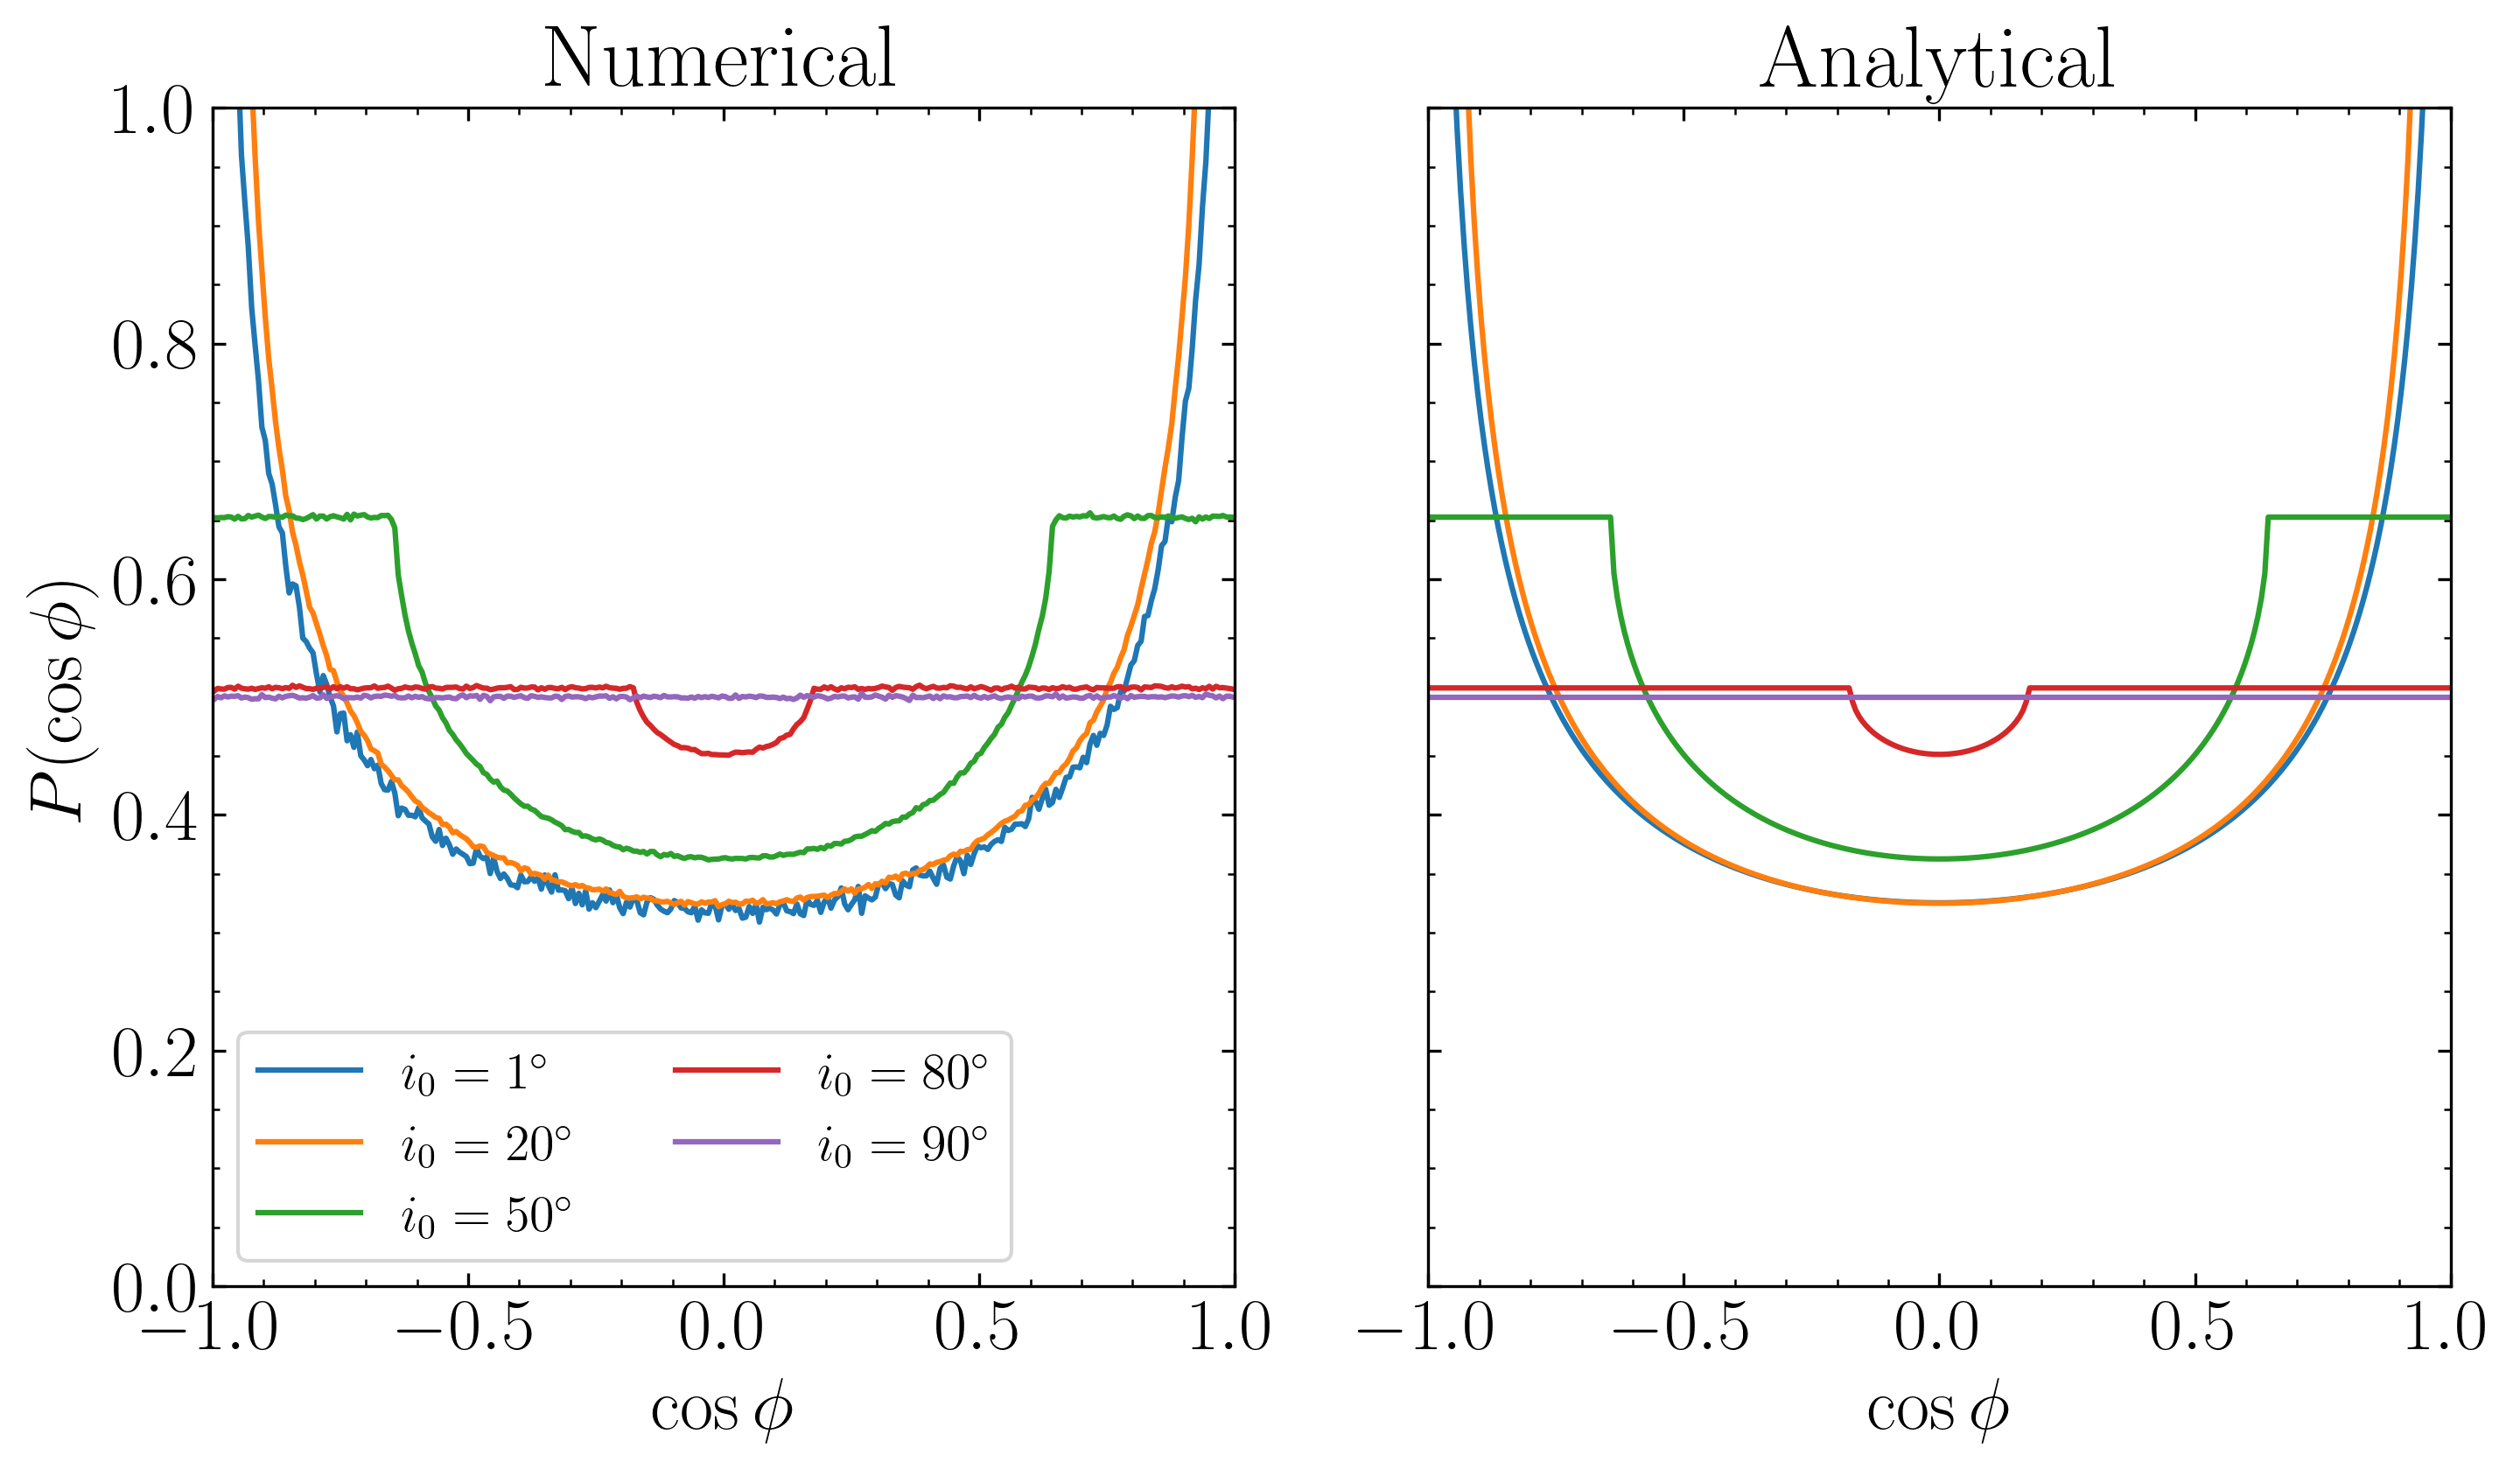
\includegraphics[width=0.7\columnwidth]{research_misc/sample_on_sphere.png}
    \caption{Numerical and analytical agreement of surface area of truncated
    unit sphere. Numerical results are from $10^8$ draws from the unit sphere
    (runs in $\sim 4$ seconds).}\label{fig:sample_on_sphere}
\end{figure}

\section{11/11/24---Love Number and Tidal Inflation}

I talked to Jeremy about this, better write it down before I forget. Inspired by
discussions with Tiger. Tldr I think his model is quite optimistic (but may be
demanded by nature), and I think that more accurate prescriptions should be
easily doable.

Consider a mini Neptune with a rocky core and envelope mass fraction $f_{\rm
env} \lesssim 10\%$ and radius $R$.
Now, inject some heat into the planet; this likely occurs at the CEB\@.
Suppose this puffs the planet up to $R'$.
What is the effect on the dynamics of the planet, most notably its $k_2$?

Recall that $k_2$ defines the induced exterior potential of the planet in
response to an external perturbation:
\begin{equation}
    \Phi_{\rm resp}\p{r > R}
        = k_2\Phi_{\rm ext}\p{\frac{R}{r}}^3
\end{equation}
Recall that $k_2 = 1.5$ for a homogeneous (uniform density) fluid, and is
something like $1$ for an $n=1$ polytrope (it can be done analytically, and I
think it's in Jeremy's notes somewhere).

Let's assume for now that $k_2$ is dominated by the planet's core.
This probably occurs as long as the core is not perfectly rigid (otherwise, it
would not deform, and $\Phi_{\rm resp} = 0$) and dominates the mass of the
planet.

If this is the case, then inflating the radius will not appreciably change the
$\Phi_{\rm resp}$.
However, the radius of the planet increased.
Thus,
\begin{equation}
    \Phi_{\rm resp}'\p{r > R'}
        = k_2'\Phi_{\rm ext}\p{\frac{R'}{r}}^3 = \Phi_{\rm resp}(r > R').
\end{equation}
Equating these two, we find that the quantity $k_2R^3$ should be conserved.

\section{11/13/24---When can Torques Overcome Accretion?}

Maybe this will go into a future paper, but I need to write it down.
This is relevant for both planetary and stellar obliquities: if it accretes from
the PPD, how can I check whether my obliquity excitation mechanisms can overcome
the accretion?

The key quantity to compare is the accreted angular momentum to the torques
(which also effect a change to the angular momentum).
While gas is accreted once it enters the Bondi radius, it cannot be added to the
star unless it loses enough angular momentum to reach the stellar surface.
Thus, I think that the specific AM of a parcel of gas that is successfully
accreted onto the host star cannot exceed the Keplerian AM at the stellar
surface, or
\begin{align}
    \mathrm{d}L
        &\lesssim \mathrm{d}m \sqrt{GMR} = R^2 \Omega_{\rm dyn} \;\mathrm{d}m,\\
    \dot{J}_{\rm acc}
        &\lesssim \dot{M} R^2\Omega_{\rm dyn}.
\end{align}
On the other hand, precessional torques have characteristic strength (e.g.\ from
a disk on equator of the star) [Lai 2014].
\begin{align}
    \bm{T}
        &\sim \frac{3GM_{\rm d}}{4r_{\rm in}^2r_{\rm out}}M_\star R_\star^2J_2.
\end{align}
Comparing these two, we find that
\begin{align}
    \frac{\dot{J}_{\rm acc}}{\bm{T}}
        &\sim \frac{4\dot{M}\sqrt{GM_\star R_\star}r_{\rm in}^2r_{\rm out}}{
            3GM_{\rm d}M_\star R_\star^2 J_2},\\
        &=
            \frac{4\dot{M}}{3M_{\rm d}\Omega_{\rm dyn}}
            \frac{r_{\rm in}^2r_{\rm out}}{R_\star^3}
            \frac{1}{J_2}.
\end{align}
Note that $J_2 = k_2 \epsilon^2 / 3$, where $\epsilon = \Omega_\star /
\Omega_{\rm dyn}$ should be $\sim 10^{-2}$ for a young star, where $\epsilon
\simeq 0.1$. Evaluating, we find
\begin{align}
    \frac{\dot{J}_{\rm acc}}{\bm{T}}
% >>> 4 / 3 * 4^2 * ((50 AU) / (2 Rsun)) * 100 / (G * Msun / (2 Rsun)^3)^(1/2) / yr
% 1636.896849
        &= \frac{10^3\mathrm{yr}}{M_{\rm d} / \dot{M}}
            \p{\frac{r_{\rm in} / R_\star}{4}}^2
            \p{\frac{r_{\rm out}}{50\;\mathrm{AU}}}
            \p{\frac{R_\star}{2R_{\odot}}}^{1/2}
            \p{\frac{M_\star}{M_{\odot}}}^{-1/2}
            \p{\frac{J_2}{10^{-2}}}^{-1}.
\end{align}
For typical values (Fig.~3 of Manara review), $\dot{M} \lesssim
10^{-8}M_{\odot}\;\mathrm{/yr}$.
As such, this expression evaluates to $\sim 10^{-4}$.
Thus, we can have a much larger inner disk truncation radius without breaking
this inequality.
In conclusion, accretion is significantly subdominant to gravitational torques
in changing the angular momentum of a young protostar.

\section{11/18/24---ZLK Fun Stuff}

\subsection{Maximum Eccentricity due to SRFs}

We start with LML15's equation evaluated at $i_0 = 90^\circ$, the maximal value
% (edit: we re-include the angular dependence for posterity, the curly braces term
% on the RHS).
\begin{align}
    \epsilon_{\rm GR} \p{\frac{1}{j_{1,\min}} - 1}
        + \frac{\epsilon_{\rm tide}}{15}
            \p{\frac{1 + 3e_{1,\max}^2 + 3e_{1,\max}^4/8}{j_{1,\min}^9} - 1}
        + \frac{\epsilon_{\rm rot}}{3}
            \p{\frac{1}{j_{1,\min}^3} - 1}
        = \frac{9}{8}\p{1 - j_{1,\min}^2}.
            % \z{1 - \frac{3\cos^2i_0}{j_{1,\min}^2}}.
\end{align}
What are the maximum eccentricities obtained when only one of the SRFs is
relevant?

Let's first do the GR case. This is simple:
\begin{align}
    \epsilon_{\rm GR} \p{\frac{1 - j_{1, \min}}{j_{1,\min}}}
        u&= \frac{9}{8} \p{1 - j_{1,\min}^2},\\
    \frac{8}{9}\epsilon_{\rm GR}
        &= j_{1,\min}\p{1 + j_{1,\min}}.
\end{align}
Since $j_{1,\min} \leq 1$, it is clear that the RHS maximizes to be $2$, and
therefore no eccentricity excitation is possible if $\epsilon_{\rm GR} \geq
9/4$. This is in agreement with Figure~6 of LML15.

What about the rotation case? This is not much harder:
\begin{align}
    \frac{\epsilon_{\rm rot}}{3} \p{\frac{1 - j_{1,\min}^3}{j_{1,\min}^3}}
        &= \frac{9}{8}\p{1 - j_{1,\min}^2},\\
    \frac{8\epsilon_{\rm rot}}{27}
        &= \frac{j_{1,\min}^3\p{1 + j_{1,\min}}}{1 + j_{1,\min} + j_{1,\min}^2}.
\end{align}
The RHS maximizes when $j_{1,\min} = 1$, where it is equal to $2/3$, and so
again no ZLK when $\epsilon_{\rm rot} \geq 9/4$.

Might as well do tides while we're here lmao. Again, we use the same idea:
$e_{1, \max} \approx 0$ when ZLK is fully suppressed, so we should just solve
\begin{align}
    \frac{\epsilon_{\rm tide}}{15}\p{\frac{1}{j_{1,\min}^9} - 1}
        &= \frac{9}{8}\p{1 - j_{1,\min}^2},\\
    \frac{8\epsilon_{\rm tide}}{135}
        &= \frac{j_{1,\min}^9\p{1 + j_{1,\min}}}{
            1 + j_{1,\min} +\dots+ j_{1,\min}^8}.
\end{align}
Again, the LHS maximizes at $1/4$, so no eccentricity excitation is obtained
when $\epsilon_{\rm tide} \geq 135/32$.

\subsection{Nonzero $e_0$ Effects}

Two questions to answer here. (i) What is the range of $e_{\max}$ for a given
$e_0$, $i_0$ and $\omega_0$, and (ii) is there such a thing as an ``inclination
window'' for finite $e_0$?

For the first one, it's clear that we just need to evaluate using the conserved
quantities. The two are:
\begin{align}
    K &= \p{1 - e^2} \cos^2i \equiv x\cos^2i,\\
    C_K
        &= e^2\p{5\sin^2i \sin^2\omega - 2}
        = \p{1 - x}\p{5\p{\frac{x - K}{x}} \sin^2\omega - 2}.
\end{align}
For a given $e_0$, the maximum $e_{\max}$ is attained when $\omega_0 = 0$ (a
circulating orbit), and the minimum $e_{\max}$ is attained when $\omega_0 = \pi$
(which can even be equal to $e_0$ if $e_0$ is below the center of the ZLK
resonance, i.e.\ the fixed point)
We can solve these two cases separately:
\begin{itemize}
    \item For the circulating case ($C_K < 0$), i.e.\ the maximum $e_{\max}$, we
        simply need to equate:
        \begin{align}
            \p{1 - x_{\min}}\s{5\p{\frac{x_{\min} - K}{x_{\min}}} - 2}
                &= -2\p{1 - x_0}\nonumber\\
            \frac{5K}{2} - \frac{3x_{\min}}{2}
                &= x_{\min}\frac{1 - x_0}{1 - x_{\min}}.
        \end{align}
        Of course, when $x_0 = 1$, this reduces to the standard ZLK result.
        Note that $x_{\min} > 0$, but the LHS must be positive as well, so $0 <
        x_{\min} < 5K/3$. Since the RHS vanishes for $x_{\min} = 0$, the LHS
        vanishes for $x_{\min} = 5K/3$, and both sides are positive, it's clear
        that by the intermediate value theorem that there will be an
        intersection that determines $x_{\min}$.
        Furthermore, if we simply rearrange
        \begin{equation}
            \frac{5K}{2} - x_{\min}\frac{1 - x_0}{1 - x_{\min}}
                = \frac{3x_{\min}}{2},
        \end{equation}
        it is clear that as $x_0$ decreases from $1$ (i.e.\ nonzero initial
        eccentricity) that the LHS decreases, thus decreasing $x_{\min}$. A
        perturbative calculation can probably give us the leading-order
        dependence if we must.

    \item For the librating case ($C_K > 0$), we instead must solve for the two
        roots of (I've included the second line to show that it's manifestly
        quadratic)
        \begin{align}
            C_K &= \p{1 - x}\s{5\p{\frac{x - K}{x}} - 2}\nonumber\\
            C_Kx &= \p{1 - x}\s{5\p{x - K} - 2x}.\label{eq:lib_cond}
        \end{align}
        I've plotted this function on Wolframalpha, but we can see the broad
        features quite easily: when $x = 0$, this function is negative (not a
        valid solution to our ``librating'' assumption), becomes positive at
        just above $x = K$, and asymptotes to $0$ again as $x \to 1$.

        Thus, for all values of $C_K > 0$ (as long as it's not too large\dots),
        there must be at least two roots, one just above $x=K$ and one out at $x
        \to 1$.
        We can hammer out the details when we need this expression, but this is
        the core result.
\end{itemize}

Now, the second point: what does it mean to have a ZLK window? Even at low
mutual inclinations, there will still be eccentricity and inclination
oscillations.
I guess what we want to describe is the window within which a libration region
appears.
But if libration is set by $C_K > 0$, we see that it is actually
\emph{eccentricity independent}, since it just depends on whether the expression
$(5\sin^2i\sin^2\omega - 2)$ exceeds zero anywhere.
Since this is maximized at $\omega = \pi/2$ of course, we recover the standard
result, that $\cos^2i < 3/5$ for $C_K > 0$!
Since when $C_K < 0$, there is only one root to Eq.~\eqref{eq:lib_cond}, it is
clear that $C_K > 0$ is indeed the condition for the ZLK resonance feature to
appear.

So then, why do eccentricity oscillations become larger in amplitude, even at
small mutual inclinations, and when we don't rely on different resonances
(coplanar ZLK, Li+14, Petrovich15)?
This must be a consequence of the circulating regime calculation.
So the question is: when $x_0$ and $K$ are comparable, but are small, what does
$x_{\min}$ look like?
We first note that
\begin{align}
    \frac{5K}{2} - \frac{5x_{\min}}{2}
        &= x_{\min}\frac{x_{\min} - x_0}{1 - x_{\min}},\\
    \frac{5}{2}\sin^2 i_{x_{\min}}
        &= \frac{x_0 - x_{\min}}{1 - x_{\min}}.
\end{align}
Note that $i_{x_{\min}}$ occurs at eccentricity maximum, which is also the
inclination minimum, and at $\omega = \pi/2$. Taking $x_{\min} \ll 1$, we can
finally arrive at
\begin{equation}
    \frac{5}{2}\sin^2 i_{\pi/2}
        \approx x_{\pi/2} - x_0.
\end{equation}
Thus, when the LHS is of order the RHS, the eccentricity cycles can still result
in substantial changes to the $x$ values. Thus, we arrive at the condition that
the inclination can still cycle due to non-resonant secular dynamics as long as
\begin{equation}
    1 - e_0^2 \lesssim \frac{5}{2}\sin^2 i_{\pi/2}.
\end{equation}

\section{12/07/24---Viscosity and Convective Front Propagation}

As Daniel [Lecoanet] rightfully points out, in Masa's simulations, the
convective front propagates due to microturbulent viscosity alone, so this
complicates the interpretation of our results somewhat.
What is the shape and rate of this propagation?
We just need to recall that
\begin{align}
    N^2 &= N^2_{\rm structure} - R_{\rm rho}^{-1}\pd{\mu}{z},\\
    \pd{\bar{\mu}}{t}
        &= \frac{\tau_0}{\mathrm{Pe}}\nabla^2\bar{\mu}
            + \dots.
\end{align}
Considering the IC as $\bar{\mu}$ being a wedge function
\begin{equation}
    \bar{\mu}
        =
        \begin{cases}
            1 & z < 1,\\
            (2 - z) & 1 < z < 2.
        \end{cases}
\end{equation}
we can pose the question: what is the rate of advance of the Ledoux-stabilized
region due to the diffusivity of the mean $\bar{\mu}$ instead?
We've neglected the $z \in [2, 3]$ region from our paper.

This can be solved analytically. Consider the 1D diffusion equation
\begin{equation}
    \pd{y}{t}
        = D\ptd{y}{x},
\end{equation}
where $D = \tau_0 / \mathrm{Pe}$ and $y = \bar{\mu}$.
Take the initial condition above.
We want to calculate where $N^2$ increases above some critical value, which is
equivalently where $\bar{\mu}$ decreases below some critical value $1 -
\epsilon$.

Let's take the second of $y_0$, which also obeys a diffusion equation
\begin{equation}
    \pd{y''}{t}
        = D\ptd{y''}{x}.
\end{equation}
$y_0''$ is a delta function $y_0'' = \delta\p{x - 1}$. It has analytic solution
to the diffusion equation (I looked this up, too lazy to do)
\begin{equation}
    y''(t, x) = \sqrt{\frac{D}{4\pi t}}\exp\s{-\frac{Dx^2}{4t}}.
\end{equation}
Thus, the analytic solution to $y'(t)$ must then be
\begin{align}
    y'(t, x)
        &= \sqrt{\frac{D}{4\pi t}}
            \int\limits_{-\infty}^x\;\mathrm{d}\xi\exp\s{-\frac{D\xi^2}{4t}}
            \nonumber\\
        &= \sqrt{\frac{1}{\pi}}
            \int\limits_{-\infty}^s\;\mathrm{d}\sigma\;e^{-\sigma^2}
            \nonumber\\
        &= \sqrt{\frac{1}{\pi}}\;\mathrm{erf}\s{x\sqrt{\frac{D}{4t}}}.
\end{align}
Not sure if I have the right definition of erf, but yeah it should be like this.
Thus, the $x$ at which $y'(t, x)$ crosses some critical $y'_{\rm crit}$ at a
given $t$ should be related to
\begin{equation}
    x_{\rm crit}
        = \sqrt{\frac{4t}{D}}\;\mathrm{erf}^{-1}\p{y'_{\rm crit}\sqrt{\pi}}
            \propto \sqrt{t}.
\end{equation}
I have trouble seeing how this can be avoided.

\section{12/09/24---Ivection Resonance and Broken Disks?}

Let's check some frequencies first. Consider a host star, binary companion,
inner and outer disk. Then
\begin{align}
    \omega_{\rm io}
        &= \frac{3}{16}\frac{m_{\rm o}}{M_\star}
            \p{\frac{r_{\rm i,out}^3}{r_{\rm o, in}^2r_{\rm o,out}}}
            n_{\rm i,out},\\
    \frac{\omega_{\rm io}}{n_{\rm b}}
        &= \frac{3}{16}\frac{m_{\rm o}}{M_\star}
            \p{\frac{r_{\rm i,out}^3}{r_{\rm o, in}^2r_{\rm o,out}}}
            \p{\frac{m_\star a_{\rm b}^3}{(m_\star + m_{\rm b})r_{\rm
            i,out}^3}}^{1/2}
                ,\\
        &\approx
            \frac{3}{16}
            \frac{m_{\rm o}}{M_\star}
            \p{\frac{r_{\rm i,out}^{3/2}a_{\rm b}^{3/2}}
                {r_{\rm o, in}^2r_{\rm o,out}}},\\
        &\approx
% >>> 3/16 * 1e-2 * (15 AU)^(3/2) * (1000 AU)^(3/2) / ((20 AU)^2 * (80 AU))
% 0.107644
            0.1
            \p{\frac{m_{\rm o} / M_\star}{10^{-2}}}
            \p{\frac{r_{\rm i,out}}{15\;\mathrm{AU}}}^{3/2}
            \p{\frac{a_{\rm b}}{10^3\;\mathrm{AU}}}^{3/2}
            \p{\frac{r_{\rm o, in}}{20\;\mathrm{AU}}}^{-2}
            \p{\frac{r_{\rm o, out}}{80\;\mathrm{AU}}}^{-1}.
\end{align}
This is if the disk obeys $\Sigma \propto r^{-1}$. But if it's a $r^{-3/2}$
disk, then\dots well, we should do this more carefully.

But also, for a $p=1$ disk, the mass is uniformly distributed $dr$. For a
$p=3/2$ disk, the local AM $2\pi r \Sigma \sqrt{r}\;\mathrm{d}r$ is uniformly
distributed.
Thus, the outer disk doesn't have much more AM than the inner disk.
Does this help us at all? TBD\@.

\section{12/17/24---IW Dissipation in Envelope}

We often hear this $(r_c/R)^5$ scaling of the IW $Q$, but can we do better in a
thin envelope? Just writing this down after chatting it through with Eliot
[Quataert].

From Ogilvie 2013 (Eq.~B3) and Barker 2020 (Eq.~39), the full tidal $Q$ for IW
should be
\begin{align}
    \frac{1}{Q'}
        = \frac{3k_2}{2Q}
        ={}&
            \epsilon^2\frac{200\pi}{189}
            \p{\frac{\alpha^5}{1 - \alpha^5}}
            \p{1 - \gamma}^2
            \p{1 - \alpha}^4\nonumber\\
        &\times
            \p{1 + 2\alpha + 3\alpha^2 + \frac{3\alpha^3}{2}}^2
            \s{1 + \p{\frac{1 - \gamma}{\gamma}}\alpha^3}\nonumber\\
        &\times
            \p{1 + \frac{3\gamma}{2}
                + \frac{5}{2\gamma}\p{1 + \frac{\gamma}{2} - \frac{3\gamma^2}{2}}
                    \alpha^3
                - \frac{9(1-\gamma)\alpha^5}{4}}^{-2}.
\end{align}
Note that this is an exact result, for the simplified two-zone model, despite
its appearance as an expansion in $\alpha$. Note that
\begin{align}
    \epsilon &= \frac{\Omega_{\star}}{\sqrt{GM_\star/R_\star^3}},&
    \alpha &= \frac{r_{\rm c}}{R},&
    \gamma &= \frac{\alpha(1 - \beta)}{\beta(1 - \alpha^3)},&
    \beta &= \frac{m_{\rm c}}{M}.
\end{align}

It's common to see this expression written as $\propto\epsilon^2\alpha^5$.
However, this only holds when $\alpha \ll 1$. In the other limit, that we're
working on with Luke, we want $\alpha \to 1$ and $\beta \to 1$, but where
$\beta$ approaches much faster. Thus, we first take the limit for $\beta \to 1$,
or $\gamma \to 0$ (if $\alpha \to 1$ slowly, certainly $\alpha^3 \to 1$ even
more slowly):
\begin{align}
    \lim_{\gamma \to 0}
        \frac{1}{Q'}
        \approx{}&
            \epsilon^2\frac{200\pi}{189}
            \p{\frac{\alpha^5}{1 - \alpha^5}}
            \p{1 - \alpha}^4\nonumber\\
        &\times
            \p{1 + 2\alpha + 3\alpha^2 + \frac{3\alpha^3}{2}}^2
            \s{\frac{\alpha^3}{\gamma}}
            \p{\frac{5\alpha^3}{2\gamma}}^{-2}\\
    \lim_{\gamma \to 0}
        \frac{1}{\gamma Q'}
        \approx{}&
            \epsilon^2\frac{200\pi}{189}
            \p{\frac{\alpha^5}{1 - \alpha^5}}
            \p{1 - \alpha}^4\nonumber\\
        &\times
            \p{1 + 2\alpha + 3\alpha^2 + \frac{3\alpha^3}{2}}^2
            \frac{4}{25\alpha^3}.
\end{align}
Now, we correspondingly take $\alpha \to 1$, and obtain
\begin{align}
    \lim_{\alpha \to 1}
        \frac{1}{\gamma Q'}
            &= \epsilon^2\frac{40\pi}{21} \p{1 - \alpha}^3,\\
    \lim_{\alpha \to 1}
    \lim_{\gamma \to 0}
        \frac{1}{Q'}
            &=
                \epsilon^2 \frac{40\pi}{21}
                \gamma \p{1 - \alpha}^3 \nonumber\\
            &=
                \epsilon^2 \frac{40\pi}{21}
                \frac{\alpha(1 - \beta)}{\beta\p{1 + \alpha + \alpha^2}}
                    (1 - \alpha)^2
                    \nonumber\\
    \lim_{r_{\rm c} \to R}
    \lim_{m_{\rm c} \to M}
        \frac{1}{Q'}
            &\approx
                \epsilon^2 \frac{40\pi}{63}
                (1 - \beta) (1 - \alpha)^2.
\end{align}

\section{02/18/25---Pseudosynchronization at High Obliquity}

Josh asked me once why pseudosynchronization is so slow at high obliquity.
To analyze this, let's look to the tidal torque along the spin axis, with all
time lags set to be equal (Eq.~27 of Lai2012):
{\small
\begin{align}
    \frac{T_z}{T_0\tau}
        &= \frac{3\pi}{20} \s{
            (1 + c)^4 (\Omega - \omega)
            + s^2(1 + c)^2(2\Omega - \omega)
            - s^2(1 - c)^2(2\Omega + \omega)
            - (1 - c)^4 (\Omega + \omega)
            }
        - \frac{3\pi}{5}
        \omega\p{s^4 + s^2c^2}.
\end{align}}
Here, $s = \sin\theta$ and $c=\cos\theta$.
When $\theta$ is close to $90^\circ$, we can set $s = 1$ and expand $c \ll 1$
to obtain
{\small
\begin{align}
    \frac{T_z}{T_0\tau}
        &\approx \frac{3\pi}{20} \s{
            (1 + 4c) (\Omega - \omega)
            + (1 + 2c)(2\Omega - \omega)
            - (1 - 2c)(2\Omega + \omega)
            - (1 - 4c) (\Omega + \omega)
            }
        - \frac{3\pi}{5} \omega\p{1 - c^4},\\
        &=
        \frac{3\pi}{20} \s{
            16c\Omega - 4\omega
            }
        - \frac{3\pi}{5} \omega\p{1 - c^4}.
\end{align}}
Setting this equal to zero, we get the usual result
\begin{equation}
    2\cos\theta = \frac{\omega}{\Omega} + \mathcal{O}\p{\cos^2\theta}.
\end{equation}
Expanding to higher order gives better precision.
But the key point is that, instead of the dominant torque being the $(22)$
component ($(1 + c)^4(\Omega - \omega)$, the only one that doesn't vanish when
$s = 0$ and $c = 1$), the only component overlapping with the orbital motion
$\Omega$ scales with $\cos\theta$ (for a highly misaligned $m'=2$ component, it
gets broken up into nearly-equal $m=\pm 2$ components, with only the
$\cos\theta$ splitting the degeneracy).
Put another way, the highly misaligned potential is much more ring-like than
orbital like, and ring-like will tend to favor zero-spin.

\section{03/21/25---Mixed Modes Maybe?}

We already know that the ``mixed modes'' Dong and I found in our Paper III are
due to high-order SORs.
These must also be identifiable in the vector formalism too though, but we can't
seem to find it.
The vector formulation is important to characterize since, when $\uv{l}$
experiences crazy evolution, no good coordinate system can be written down.

We will approximate a bit.
Consider the inertial frame equations
\begin{align}
    \rd{\uv{s}}{t}
        &=
            \alpha\p{\uv{s} \cdot \uv{l}}
                \p{\uv{s} \times \uv{l}},\\
    \uv{l}
        &\approx
            \uv{z}
            + \Re(\mathcal{I}) \uv{x}
            + \Im(\mathcal{I}) \uv{y},\\
    \mathcal{I}
        &=
            I_1e^{ig_1t}
            + I_2e^{ig_2t}.\label{eq:dsdt_inertial}
\end{align}

\subsection{Total AM approach}

Let's instead adopt the celestial mechanics approach, where we keep the total AM
$\uv{l}_{\rm p}$ along the $z$-axis.

Start again from the inertial frame equations, Eq.~\eqref{eq:dsdt_inertial}.
Consider a rotation with rate $\bar{g}$.
\begin{align}
    \p{\rd{\uv{s}}{t}}'
        &=
            \alpha\p{\uv{s} \cdot \uv{l}}
                \p{\uv{s} \times \uv{l}}
            + \bar{g}\p{\uv{s} \times \uv{z}}
                ,\\
    \mathcal{I}
        &=
            I_1e^{i(g_1 - \bar{g})t}
            + I_2e^{i(g_2 - \bar{g})t}.
\end{align}
This problem is somewhat difficult because $\uv{l}$ contains two parameters:
$I_2 \ll I_1 \ll 1$, the last expressing the point that $\uv{l} \approx \uv{z}$.
Denote $\uv{s}_{ij}$ to be $i$th order in $I_1$ and $j$th order in $I_2$

Let's first evaluate the ODE at the lowest order, $\uv{l} \approx \uv{z}$:
\begin{align}
    \rd{\uv{s}_{00}}{t}
        &=
            \alpha\p{\uv{s}_{00} \cdot \uv{z}}
                \p{\uv{s}_{00} \times \uv{z}}
            + \bar{g}\p{\uv{s}_{00} \times \uv{z}},\\
    \alpha \p{\uv{s}_{00} \cdot \uv{z}} &= -\bar{g}.
\end{align}
This is the simple result.

Now, what about at leading order in $I_1$, assuming $I_2 = 0$?
Note that the next-order correction to $\uv{s}$, denoted $\uv{s}_{10}$, is not a
unit vector.
\begin{align}
    \rd{\bm{s}_{10}}{t}
        ={}&
            \alpha
                \p{\bm{s}_{10} \cdot \uv{z}}
                \p{\uv{s}_{00} \times \uv{z}}
            + \cancel{\alpha
                \p{\uv{s}_{00} \cdot \uv{z}}
                \p{\bm{s}_{10} \times \uv{z}}
            + \bar{g}\p{\bm{s}_{10} \times \uv{z}}}\nonumber\\
        &+ \alpha
                \p{\uv{s}_{00} \cdot \bm{l}_{\perp}}
                \p{\uv{s}_{00} \times \uv{z}}
            + \cancelto{-\bar{g}}{\alpha
                \p{\uv{s}_{00} \cdot \uv{z}}}
                \p{\uv{s}_{00} \times \bm{l}_{\perp}}.\label{eq:ds10dt}
\end{align}
Note now that $\bm{s}_{10}$ is not constant.
We expect it to look like a uniformly rotating matrix though, so let's demand
that
\begin{equation}
    \rd{\bm{s}_{10}}{t} = \bm{\omega} \times \uv{s}_{10},
\end{equation}
where $\bm{\omega} \perp \bm{s}_{10}$.

There is one solution.
Let's guess that $\bm{\omega} \propto \uv{s}_{00}$, and $\bm{s}_{10}$ oscillates
in phase with $\bm{l}_{\perp}$, i.e.\
\begin{align}
    \bm{s}_{10} &\propto \bm{l}_{\perp} - \p{\uv{s}_{00} \cdot \bm{l}_{\perp}}
        \uv{s}_{00},\\
    \bm{\omega} &= -\bar{g}\uv{s}_{00},\label{eq:s10_prec}
\end{align}
The amplitude of $\bm{s}_{10}$ is fixed by demanding that the first two terms in
Eq.~\eqref{eq:ds10dt} cancel:
\begin{align}
    0 &= \bm{s}_{10} \cdot \uv{z} + \uv{s}_{00} \cdot \bm{l}_{\perp},\\
        &= C\p{\uv{s}_{00} \cdot \bm{l}_{\perp}}
            \frac{\bar{g}}{\alpha}
            + \uv{s}_{00} \cdot \bm{l}_{\perp},\\
    C &= -\frac{\alpha}{\bar{g}},\\
    \bm{s}_{10}
        &= -\frac{\alpha}{\bar{g}}
            \s{\bm{l}_{\perp} - \p{\uv{s}_{00} \cdot \bm{l}_{\perp}}
        \uv{s}_{00}}.
\end{align}
Thus, indeed such a solution for $\bm{s}_{10}$ exists.

Now, note that $\bm{s}_{10}$ has time-varying components along
$\bm{l}_{\perp}$ (implying oscillation frequencies $(g_1 - \bar{g})$ and $(g_2 -
\bar{g})$), while its rotation has frequency $\bar{g}$ (Eq.~\ref{eq:s10_prec}).
Consistency among all of these frequencies demands $\bar{g} = (g_1 +
g_2) / 2$ (excepting the trivial solutions $\bar{g} = g_1$ and $g_2$).

Looking back at my paper, it looks like we can have $\bm{s}_{10}$ oscillate in
the $xy$ plane, just with no $z$ component.
But this makes sense: the $z$ component oscillation is just because the true
$z$ axis should be $\uv{l}$, not $\uv{l}_{\rm p}$.
So our $\bm{s}_{10}$ should be such that
\begin{align}
    \p{\uv{s}_{00} + \bm{s}_{10}} \cdot \p{\uv{z} + \bm{l}_{\perp}}
        &= \uv{s}_{00} \cdot \uv{z}
            + \frac{\alpha}{\bar{g}}\p{\uv{s}_{00} \cdot \bm{l}_{\perp}}
                \uv{s}_{00} \cdot \uv{z}
            + \uv{s}_{00} \cdot \bm{l}_{\perp},\\
        &= \uv{s}_{00} \cdot \uv{z}.
\end{align}
Yay!

Well, I guess at this point, we've successfully shown that $\bm{s}_{10}$ must
have an azimuthal component $\sim \mathcal{O}\p{I_1}$, and the polar component
must be $\lesssim \mathcal{O}\p{I_2}$ (which it is), and the frequency of
oscillation still does demand that $\bar{g} = g_1 - \bar{g} = -g_2 + \bar{g}$.
Is this enough? Maybe we should expand to one more order, $\bm{s}_{01}$, to show
that we've truly found the correct state\dots

\subsection{Co-precessing, co-nutating approach}

\textbf{For posterity, I include the erroneous approach I started with\dots}

We will go to the co-precessing, co-nutating frame, and point $\uv{z}$ along the
vertical axis.
This means that $\uv{l} \to \uv{z}$ while $\uv{l}_{\rm p} = \uv{z} \to -\uv{l}$.
So
\begin{align}
    \p{\rd{\uv{s}}{t}}_{\rm co-p}
        &=
            \alpha\p{\uv{s} \cdot \uv{z}}
                \p{\uv{s} \times \uv{z}}
                - \dot{\Omega}\p{\uv{l}_{\rm p} \times \uv{s}}
                - \dot{I}\s{\p{\uv{l}_{\rm p} \times \uv{z}} \times \uv{s}}
                ,\\
    \uv{l}_{\rm p}
        &\approx
            \uv{z}
            - \abs{\mathcal{I}} \uv{x}
\end{align}
Note that $\dot{\Omega}$ has contributions from both modes, but $\dot{I} \sim
\mathcal{O}(I_2 / I_1)$ is small in amplitude.
While there are a lot more terms (and this looks ugly), it will be easier to do
expansions since there are no crazy cross terms with $s^2l^2$.
Of course, in the limit $I_2 = 0$, we have $\dot{I} = 0$ and we recover the
standard CS EOM\@.

Note that in the limit $I_2 \ll I_1$, we should have that
\begin{align}
    \Omega
        &=
            \arctan\p{\frac{I_1 \sin g_1t + I_2\sin g_2t}{I_1\cos g_1t + I_2\cos
            g_2t}},\\
        &\approx
            \arctan\p{\tan g_1t
                + \frac{I_2\cos g_2t}{I_1\cos g_1t}\p{\tan g_2t - \tan g_1t}},\\
        &\approx
            g_1t +
                \frac{I_2 \cos g_1t\cos g_2t}{I_1}\p{\tan g_2t - \tan g_1t}
                    \nonumber\\
        &= g_1t +
                \frac{I_2}{I_1}\sin\p{g_2 - g_1}t,\\
    \dot{\Omega} &= g_1 + \Delta g\frac{I_2}{I_1}\sin\Delta gt,
\end{align}
while
\begin{align}
    I(t)
        &=
            \p{I_1^2 + I_2^2 \cos\p{g_2 - g_1}t}^{1/2},\\
        &\approx
            I_1
                + \frac{I_2^2}{2I_1^2}\cos\p{g_2 - g_1}t,\\
    \dot{I}
        &= \Delta g\frac{I_2^2}{2I_1^2}\cos\Delta gt.
\end{align}

Now, let's consider further rotating into a new reference frame.
Consider a rotation by some $-\bar{g}$ (which we will later set to be $-(g_1 +
g_2) / 2$):
\begin{align}
    \p{\rd{\uv{s}}{t}}_{\rm co-p}
        &=
            \alpha\p{\uv{s} \cdot \uv{z}}
                \p{\uv{s} \times \uv{z}}
                - \dot{\Omega}\p{\uv{l}_{\rm p} \times \uv{s}}
                - \dot{I}\s{\p{\uv{l}_{\rm p} \times \uv{z}} \times \uv{s}}
                + \bar{g}\p{\uv{z} \times \uv{s}}
                \label{eq:dsdt_toexpand}
                ,\\
    \uv{l}_{\rm p}
        &\approx
            \uv{z}
            - \Re(\mathcal{I}) \uv{x}
            - \Im(\mathcal{I}) \uv{y},\\
    \mathcal{I}
        &=
            Ie^{i\bar{g}t}.
\end{align}

At leading order, $\uv{l}_{\rm p} \approx \uv{z}$, while $\dot{\Omega} \approx
g_1$ (this may not be the dominant term by magnitude, but in a time-averaged
sense the $g_2I_2$ contribution vanishes), and $\dot{I} \approx 0$, and we
obtain
\begin{equation}
    \rd{\uv{s}_0}{t}
        =
            \alpha\p{\uv{s}_0 \cdot \uv{z}}
                \p{\uv{s}_0 \times \uv{z}}
                - g_1\p{\uv{z} \times \uv{s}}
                + \bar{g}\p{\uv{z} \times \uv{s}}.
\end{equation}
This admits constant solutions if $\uv{s}_0 \cdot \uv{z} = (g_1 - \bar{g}) /
\alpha$.
Easy enough.
In order for there to be librating solutions, let's further demand that
$\uv{s}_0$ be in the $\uv{x}$--$\uv{z}$ plane.

What about the next order terms?
(there should be seven, because in Eq.~\ref{eq:dsdt_toexpand}, the first term
has two terms that depend on $\uv{s}$, the second term has three terms that have
leading order behavior, the third term is small so only contributes one term at
leading (small) order, and the fourth only needs to be expanded in $\uv{s}$)
\begin{align}
    \rd{\uv{s}_1}{t}
        ={}&
            \alpha\p{\uv{s}_1 \cdot \uv{z}}
                \p{\uv{s}_0 \times \uv{z}}
            + \cancel{\alpha\p{\uv{s}_0 \cdot \uv{z}}
                \p{\uv{s}_1 \times \uv{z}}}
                - \frac{\Delta gI_2}{I_1}\sin\Delta g t
                    \p{\uv{z} \times \uv{s}_0}
                - \cancel{g_1\p{\uv{z} \times \uv{s}_1}}\nonumber\\
            &- g_1\p{\uv{l}_{\rm p, \perp} \times \uv{s}_0}
                - \Delta g\frac{I_2^2}{2I_1^2}\cos\Delta gt
                    \s{\p{\uv{l}_{\rm p} \times \uv{z}} \times \uv{s}_0}
                + \cancel{\bar{g}\p{\uv{z} \times \uv{s}_1}}.
\end{align}
The cancelled terms vanish from the zeroth order term, so
\begin{align}
    \rd{\uv{s}_1}{t}
        ={}&
            \alpha\p{\uv{s}_1 \cdot \uv{z}}
                \p{\uv{s}_0 \times \uv{z}}
                - \frac{\Delta gI_2}{I_1}\sin\Delta g t
                    \p{\uv{z} \times \uv{s}_0}\nonumber\\
            &- g_1\p{\uv{l}_{\rm p, \perp} \times \uv{s}_0}
                - \Delta g\frac{I_2^2}{2I_1^2}\cos\Delta gt
                    \s{\p{\uv{l}_{\rm p, \perp} \times \uv{z}} \times \uv{s}_0}.
\end{align}
Note that $(\uv{l}_{\rm p, \perp} \times \uv{z}) \times \uv{s}_0 =
\uv{z}\p{\uv{l}_{\rm p, \perp} \cdot \uv{s}_0} - \uv{l}_{\rm p, \perp}(\uv{s}
\cdot \uv{z})$.

The first two terms point along the $\uv{y}$ axis, while the last two point
along all three.
The third term is much larger in magnitude than the fourth term though, so its
non-$\uv{y}$ contributions must be cancelled by corrections to the zeroth-order
solution.
From this, we see that $\uv{s}_1 \times \uv{z}$ must have a $\bar{g}$ time
dependence.
But the first two terms immediately show that $\uv{s}_1$ must have a $\Delta g$
time dependence.
Thus, we recover that $\bar{g} = \pm \Delta g$.
We've just shown that the other first-order solution are the mode-2 Cassini
States!
That won't do.

The reason is obvious: the spin-orbit resonance we were looking for must exist
at higher order, and we've only taken our expansion up to first order.
To expand this to second order would be quite a lengthy task.

\end{document}

